\documentclass[12pt]{beamer}

\usetheme{Air}
\usepackage{thumbpdf}
\usepackage{wasysym}
\usepackage{ucs}
\usepackage[utf8]{inputenc}
\usepackage{pgf,pgfarrows,pgfnodes,pgfautomata,pgfheaps,pgfshade}
\usepackage{verbatim}

\usepackage{gitinfo2}
\usepackage{tikz}
\usepackage{subfig}

\usepackage[absolute,overlay]{textpos}
\usepackage{graphicx}

\usetikzlibrary{fadings}
\usetikzlibrary{positioning}
\usetikzlibrary{arrows, matrix}

\makeatletter
\newbox\@backgroundblock
\newenvironment{backgroundblock}[2]{%
  \global\setbox\@backgroundblock=\vbox\bgroup%
    \unvbox\@backgroundblock%
    \vbox to0pt\bgroup\vskip#2\hbox to0pt\bgroup\hskip#1\relax%
}{\egroup\egroup\egroup}
\addtobeamertemplate{background}{\box\@backgroundblock}{}
\makeatother



\pdfinfo
{
  /Title       (What limits fire, where and when?)
  /Creator     (CEH)
  /Author      (Douglas Kelley - douglas.i.kelley@gmail.com)
}

\title{What limits fire, where and when?}
\subtitle{Sensitivity of burnt area to different controls}
\author{Douglas Kelley, Ioannis Bistinas, Rhys Whitley, Toby Marthews, Chantelle Burton}
\date{14th March 2017}

\titlegraphic{
\includegraphics[width=3.0cm]{logos/cehlogo945}\hspace*{1.6cm}~%
              
\includegraphics[width=1.5cm]{logos/ukesm-logo}\hspace*{1.6cm}~%
              
\includegraphics[width=3.0cm]{logos/nerc-long-logo-large}

              %\tiny{url: https://github.com/douglask3/LimFIRE ---
              %      revision no: \gitAbbrevHash}
             }

\begin{document}

\frame{\titlepage}

%\section*{}
%\begin{frame}
%  \frametitle{Outline}
%  \tableofcontents[section=1,hidesubsections]
%\end{frame}

%\AtBeginSection[]
{
  \pgfdeclareimage[width=1.0\paperwidth]{header-image}{header_images/fire}
%  \frame<handout:0>
%  {
%    \frametitle{Outline}
%    \tableofcontents[currentsection,hideallsubsections]
%  }
}

%\AtBeginSubsection[]
%{
%  \frame<handout:0>
%  {
%    \frametitle{Outline}
%    \tableofcontents[sectionstyle=show/hide,subsectionstyle=show/shaded/hide]
%  }
%}\textsl{}

\newcommand<>{\highlighton}[1]{%
  \alt#2{\structure{#1}}{{#1}}
}

\newcommand{\icon}[1]{\pgfimage[height=1em]{#1}}


%%%%%%%%%%%%%%%%%%%%%%%%%%%%%%%%%%%%%%%
%%%%%%%%%% Content starts here %%%%%%%%%%
%%%%%%%%%%%%%%%%%%%%%%%%%%%%%%%%%%%%%%%%%

\section{Introduction}
\pgfdeclareimage[width=1.0\paperwidth]{header-image}{header_images/kata_tjuta}

\begin{frame}
    \frametitle{It burns where it rains}
    \framesubtitle{Unimodal relationship with moisture}

    \foreach \x in {1, 2, 3, 4, 5, 6, 7, 8, 9, 10, 11, 12} {
        \only<\x> {
        \begin{textblock*}{10cm}(0cm,1.5cm)
            \includegraphics[width=13.0cm]{images/unimodal/p\x.png}%images/unimodal/p\x.png}
    \end{textblock*}
    }}
    %Make clear we are talking about burnt area
\end{frame}

\begin{frame}<1-3>[label = intro]
    \frametitle{What else controls fire?}
    \framesubtitle{Is it Ignitions? Is it people?}
	\begin{itemize}
		\visible<2-> {\item Fire-vegetation models incorporate ignition schemes}
		\visible<3-> {\item Schemes often include human and lightning caused ignitions}
		\visible<4-> {\item All models with human-caused ignitions show increased burnt area with people}
		\visible<5-> {\item Little effort placed in anthropagenic fire suppression}
	\end{itemize}

\end{frame}

\begin{frame}
    \frametitle{What else controls fire?}
    \framesubtitle{Is it Ignitions? Is it people?}
    FireMIP slide from Stijn
    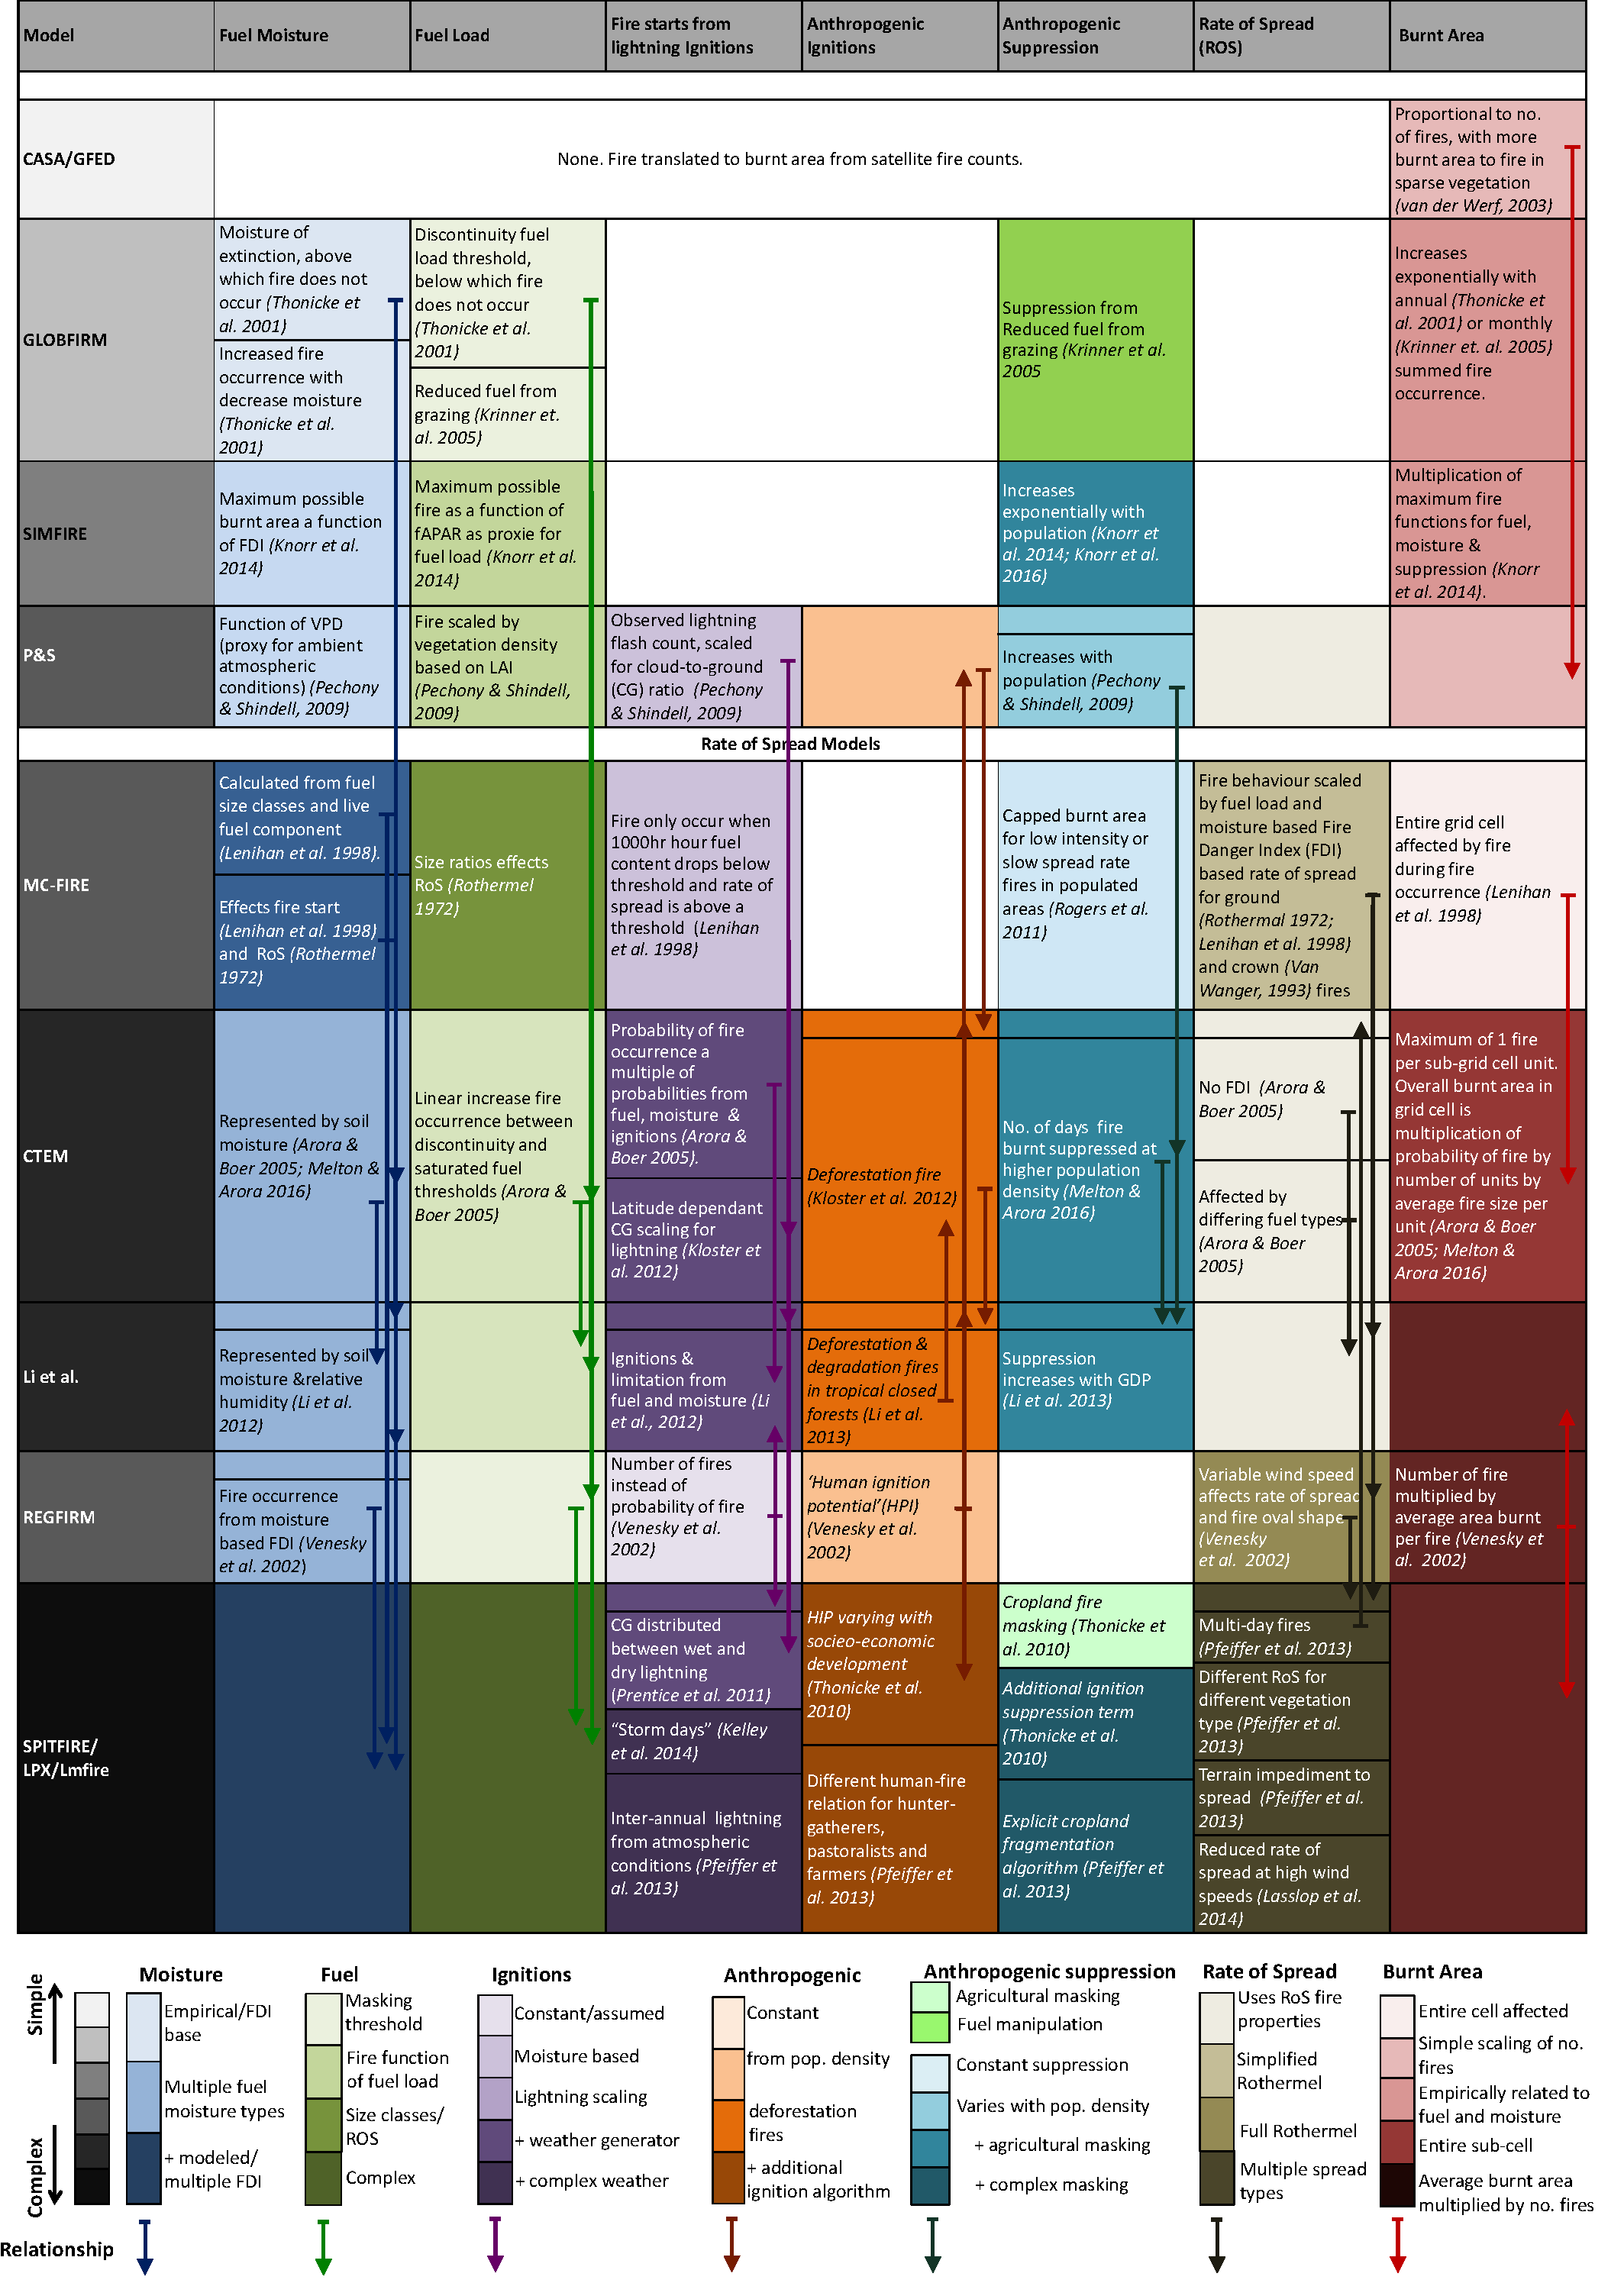
\includegraphics[width=3cm]{images/Table1.pdf}%images/unimodal/p\x.png}
\end{frame}

\againframe<3-4>{intro}

\begin{frame}
    \frametitle{What else controls fire?}
    \framesubtitle{Is it Ignitions? Is it people?}
    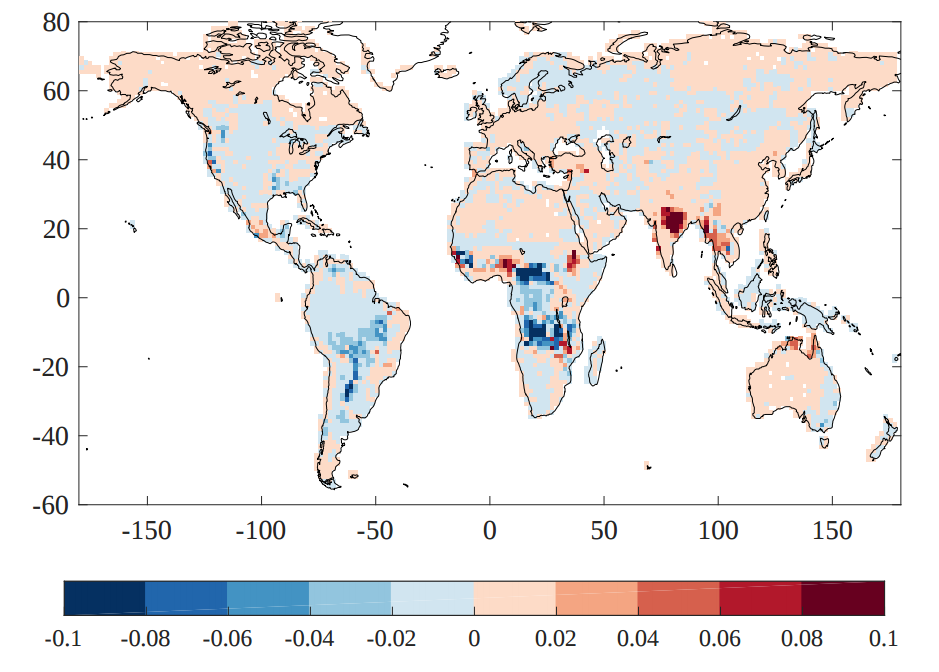
\includegraphics[width=9.0cm]{images/INFERNO}%images/unimodal/p\x.png}
	%Inferno plot
\end{frame}

\againframe<4->{intro}

\begin{frame}
    \frametitle{What else controls fire?}
    \framesubtitle{Fire-limitation framework}
	\begin{itemize}
		\visible<2-> {\item Map the limitation and sensitivity of burnt area to}
        \begin{itemize}
            \visible<3-> {\item Fuel discontinuity}
            \visible<4-> {\item Fuel moisture and atmospheric drying potential}
            \visible<5-> {\item lightning and human ignitions}
            \visible<6-> {\item land use and human suppression}
        \end{itemize}
		\visible<7-> {\item Controls are described from remote sensed and meteorological observations}
		\visible<8-> {\item optimized againstburnt area observations}
	\end{itemize}
\end{frame}

\section{Methods}
\pgfdeclareimage[width=1.0\paperwidth]{header-image}{header_images/Sierra_Calderona}

\def \inputMap#1#2#3#4 {
    \begin{backgroundblock}{#1}{#2}
        \begin{tikzpicture}
            \node[anchor=south west,inner sep=0] (image) at (0,0) {
                \includegraphics[width=4.0cm]{images/inputs/#3}
            };
            \node[align=center, font = {\tiny}] at (2.15cm, 2.33cm) {#4};
        \end{tikzpicture}
    \end{backgroundblock}
}

\def \inputMapA#1#2 {
    \inputMap{5cm}{1.33cm}{#1}{#2}
}
\def \inputMapB#1#2 {
    \inputMap{6.67cm}{3.67cm}{#1}{#2}
}
\def \inputMapC#1#2 {
    \inputMap{8.33cm}{6cm}{#1}{#2}
}

\begin{frame}<2-5>[label=framework]
    \frametitle{Fire limitation framework}
    \framesubtitle{Spatial and Temporal controls on burnt area}

    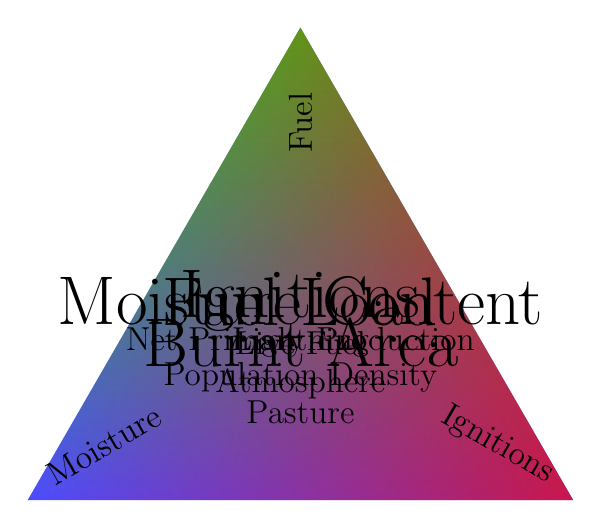
\begin{tikzpicture}
        \visible<2->{\fill[blue , opacity = 0.7] (90:4) -- (210:4) -- (-30:4) -- cycle;}
        \visible<3->{\fill[green,path fading=south, opacity = 0.85] (90:4) -- (210:4) -- (-30:4) -- cycle;}
        \visible<4->{\fill[red  ,path fading=west, opacity = 0.7] (90:4) -- (210:4) -- (-30:4) -- cycle;}

       
        \visible<2>{
            \node (note) at (0, 1.5em) {\Huge Moisture Content};
            \node (note) at (0, 0.0em) {\large Live Fuel};
            \node (note) at (0,-1.5em) {\large Atmosphere};
        }

        \visible<3->{
            \node[rotate = 30] at (-2.5, -1.3) {\large Moisture};
        }
    
	     \visible<3>{
	    	\node (note) at (0,1.5em) {\Huge Fuel Load};
	    	\node (note) at (0,0) {\large Net Primary Production};
	    }
	    
	   % \visible<4->{
	   % 	\node[rotate = -30] at (2.6,-1.3) {\large Fuel};
	    %	\node[rotate = -30] at (2.4,-1.6) {NPP};
	   % }	
    
	    \visible<4->{
	    	\node[anchor = east, rotate = 90] at (0, 3.3) {\large Fuel};
	    }
    
        \visible<4>{
            \node (note) at (0,1.5em) {\Huge Ignitions};
            \node (note) at (0,0) { \large Lightning};
            \node (note) at (0,-1.25em) { \large Population Density};
            \node (note) at (0,-2.5em) { \large Pasture};
        }

        \visible<5->{
           \node[rotate = -30] at (2.5, -1.3) {\large Ignitions};
        }

        \visible<5>{
            \node (note) at (0,0) {\Huge Burnt Area};
        }

    \end{tikzpicture}

    \begin{textblock*}{5cm}(6.67cm,2cm)
        \visible<7->{
            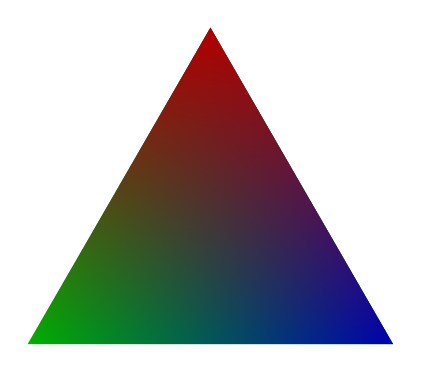
\begin{tikzpicture}[scale=0.67]
                \fill[green] (90:4) -- (210:4) -- (-30:4) -- cycle;
                \fill[blue,path fading=west] (90:4) -- (210:4) -- (-30:4) -- cycle;
                \fill[red,path fading=south] (90:4) -- (210:4) -- (-30:4) -- cycle;
                \fill[black, opacity = 0.3] (90:4) -- (210:4) -- (-30:4) -- cycle;
            \end{tikzpicture}
        }
    \end{textblock*}

    \begin{textblock*}{5cm}(10.1cm,2cm)
        \visible<7->{
            
\begin{tikzpicture}[scale=0.33]
                \fill[green] (90:4) -- (210:4) -- (-30:4) -- cycle;
                \fill[blue,path fading=west] (90:4) -- (210:4) -- (-30:4) -- cycle;
                \fill[red,path fading=south] (90:4) -- (210:4) -- (-30:4) -- cycle;
                \fill[black, opacity = 0.5] (90:4) -- (210:4) -- (-30:4) -- cycle;
            \end{tikzpicture}
        }
    \end{textblock*}

    \begin{textblock*}{4.5cm}(4.6cm,2.6cm)
        \visible<7->{
            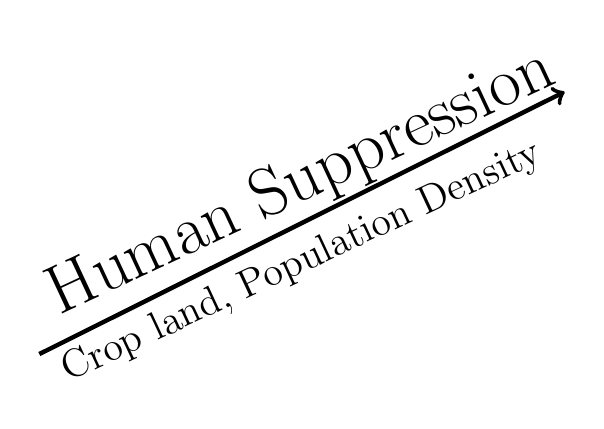
\begin{tikzpicture}
                \node[rotate = 25 ] (note) at (3.335, 2.165) {\Huge Human Suppression};
                    \node[rotate = 25 ] (note) at (3.335, 1.165) {\Large Crop land, Population Density};
                \draw[ultra thick, ->] (0, 0) -- (6.67, 3.33);
            \end{tikzpicture}
        }
    \end{textblock*}

	\only<2> {
		\inputMap{5cm}{1.18cm}{inputs_mean-alpha}{STASH $\frac{Actual}{Potential}$ Evapotranspiration \\ (Whitley et al 2014; Davis et al 2016)}
		\inputMapB{inputs_mean-emc}{Equilibrium Fuel Moisture Content}
	}


    \only<3> {
        \inputMapA{inputs_mean-npp}{MODIS NPP (MODIS 17)}
    }

    \only<4> {
        \inputMapA{inputs_mean-Lightn}{LIS/OTD (Christian 1999)}
        \inputMapB{inputs_mean-popdens}{HYDE Popdens (Goldewijk  et al 2011)}
        \inputMapC{inputs_mean-pas}{HYDE Pasture (Goldewijk et al 2011)}
    }

	\only<7> {
		\inputMap{4.7cm}{1.33cm}{inputs_mean-popdens}{HYDE Popdens (Goldewijk et al 2011)}
		\inputMap{8.33cm}{6cm}{inputs_mean-crop}{HYDE crop (Goldewijk et al 2011)}
	}

    \only<5> {
    	\begin{backgroundblock}{4.2cm}{1.33cm}
    		\begin{tikzpicture}
		         \node[anchor=south west,inner sep=0] (image) at (0,0) {
		        	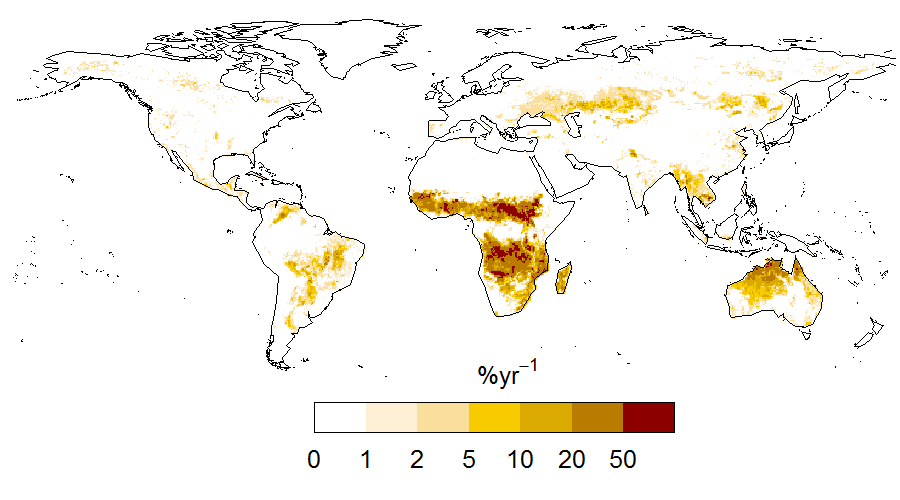
\includegraphics[width=7.0cm]{images/inputs/inputs_mean-fire}
		        };
		        \node[align=center, font = {\small}] at (2.95cm, 4.2cm) {Global Fire Emission Database 4s \\ (Giglio et al 2013; Randerson et al 2012)};
	        \end{tikzpicture}
	    \end{backgroundblock}
        %?% Make bigger
    }
    %?% Stuff to include:
    %?%   Monthly -> Inter annual and seasonal controls
\end{frame}

\def \controlsSide#1 {
    \begin{textblock*}{11cm}(0cm,1.5cm)
        \begin{tikzpicture}
            \node[anchor=south west,inner sep=0] (image) at (0,0) {
                \includegraphics[width=13.0cm]{images/#1}
            };
            \visible<-4> {\draw[white, fill = white] (6.5,3.0) -- (13.0,3.0) -- (13.0,7) -- (6.5,7) -- (6.5,3.0);}
            \visible<-1> {\draw[white, fill = white] (0.0,0.0) -- ( 6.5,0.0) -- ( 6.5,3.5) -- (0.0,3.5) -- (0.0,0.0);}
           \visible<-4>  {\draw[white, fill = white] (6.5,3.0) -- (13.0,3.0) -- (13.0,0.0) -- (6.5,0.0) -- (6.5,3.0);}
            %\visible<-4> {\draw[white, fill = white] (0.0,0) -- (12.0,0) -- (12.0,1.0) -- (0.0,1.0) -- (0.0,0);}
        \end{tikzpicture}
    \end{textblock*}
    \begin{textblock*}{11cm}(2.0cm, 7.5cm)
        \includegraphics[width=5.0cm]{images/#1_legend}
    \end{textblock*}
}

\pgfdeclareimage[width=1.0\paperwidth]{header-image}{header_images/kata_tjuta}

\begin{frame}
	\frametitle{Controls on fire}
	%\framesubtitle{Geographic controls}
	\begin{textblock*}{14cm}(0.3cm,1.2cm)
		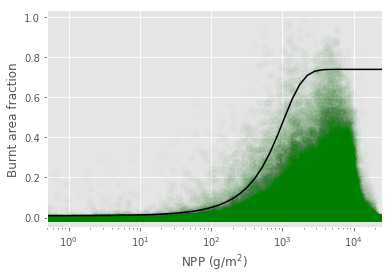
\includegraphics[width=5.78cm]{images/limitCurves/NPPVsFire}	
	\end{textblock*}
	\begin{textblock*}{14cm}(6.5cm,1.2cm)
		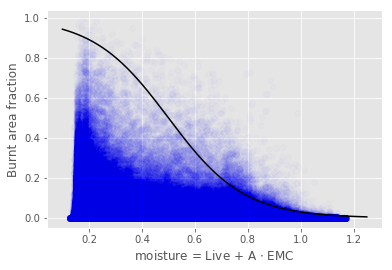
\includegraphics[width=5.78cm]{images/limitCurves/alphaVsFire}	
	\end{textblock*}
	\begin{textblock*}{14cm}(0.32cm,5cm)
		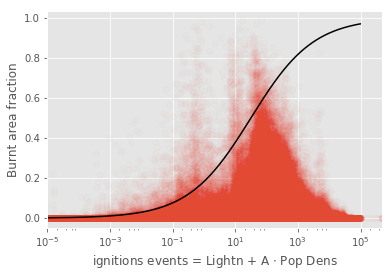
\includegraphics[width=5.78cm]{images/limitCurves/ignitionsVsFire.png}		
	\end{textblock*}
	\begin{textblock*}{14cm}(6.5cm,5.3cm)
		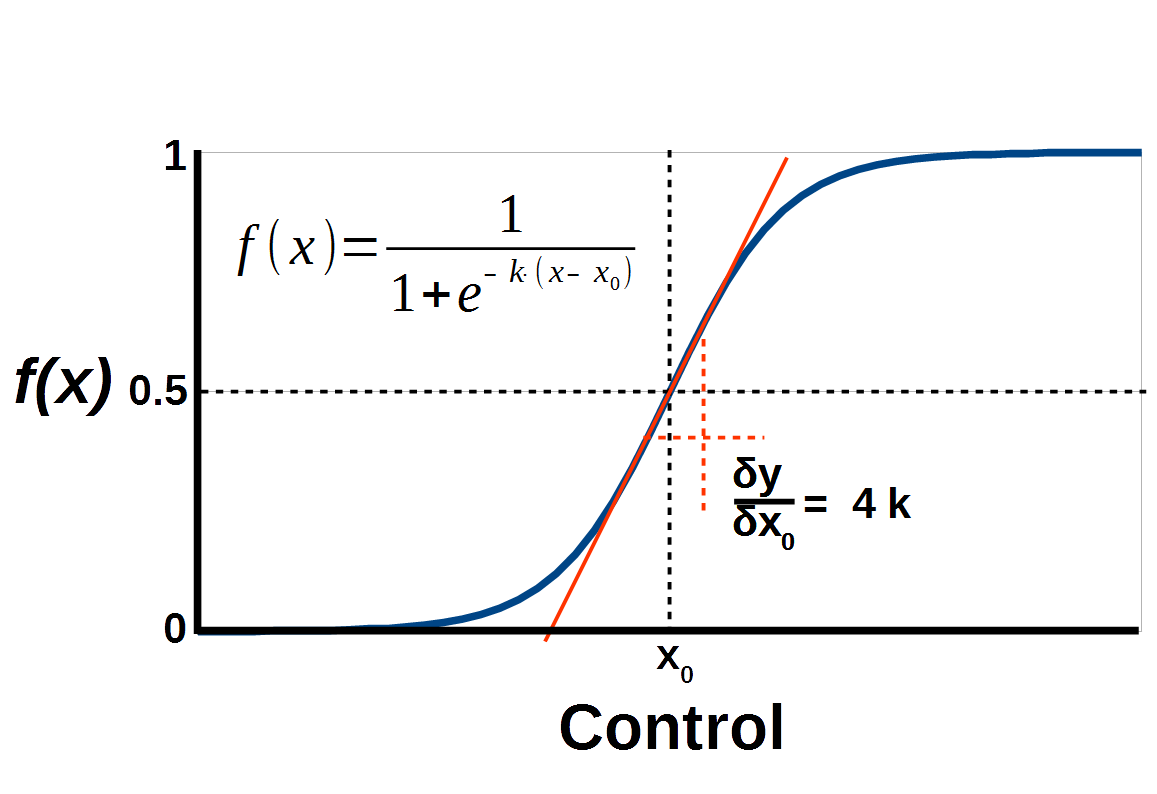
\includegraphics[width=5.78cm]{../diagrams/Logistic_fun.png}		
	\end{textblock*}
\end{frame}
\addtocounter{framenumber}{-1}

\begin{frame}
	\frametitle{Controls on fire}
	%\framesubtitle{Geographic controls}
	\begin{textblock*}{14cm}(0.3cm,1.2cm)
		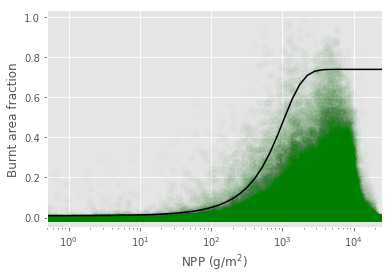
\includegraphics[width=5.78cm]{images/limitCurves/NPPVsFire}	
	\end{textblock*}
	\begin{textblock*}{14cm}(6.5cm,1.2cm)
		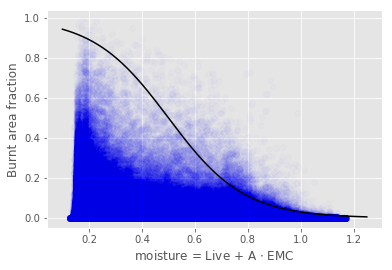
\includegraphics[width=5.78cm]{images/limitCurves/alphaVsFire}	
	\end{textblock*}
	\begin{textblock*}{14cm}(0.32cm,5cm)
		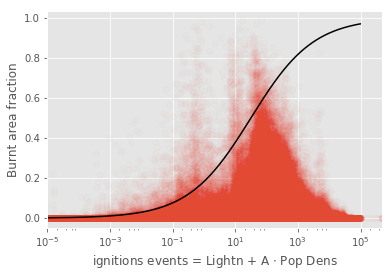
\includegraphics[width=5.78cm]{images/limitCurves/ignitionsVsFire.png}		
	\end{textblock*}
	\begin{textblock*}{14cm}(6.5cm,5.3cm)
		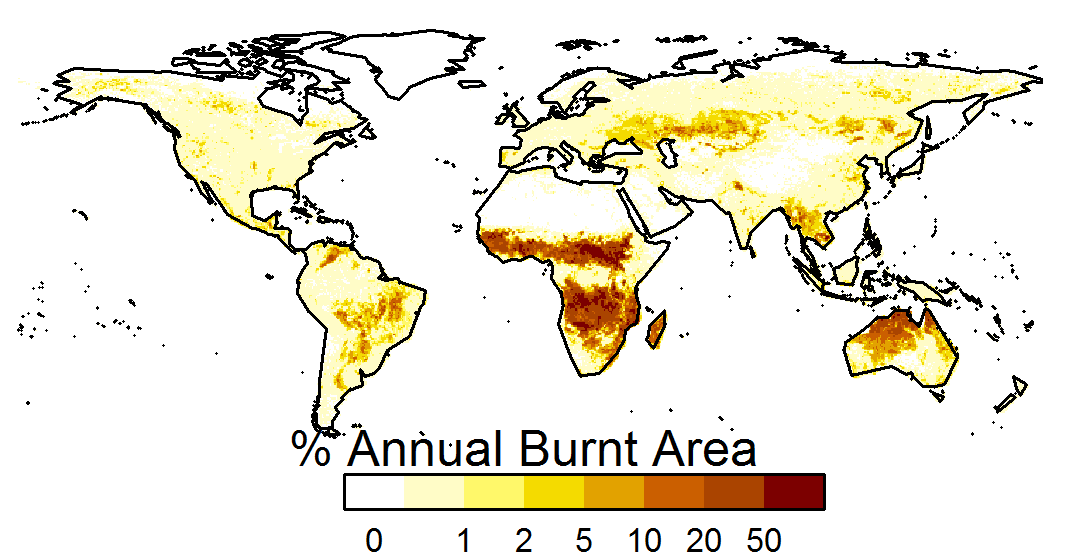
\includegraphics[width=5.78cm]{images/limitCurves/fireMap.png}		
	\end{textblock*}
\end{frame}
\addtocounter{framenumber}{-1}

\begin{frame}
	\frametitle{Controls on fire}
	%\framesubtitle{Geographic controls}
	\begin{textblock*}{14cm}(0.3cm,1.2cm)
		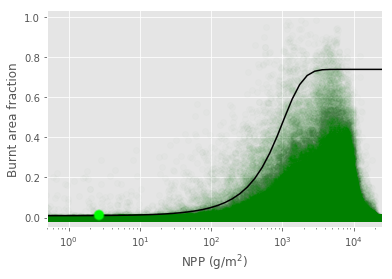
\includegraphics[width=5.78cm]{images/limitCurves/Desert/NPPVsFire}	
	\end{textblock*}
	\begin{textblock*}{14cm}(6.5cm,1.2cm)
		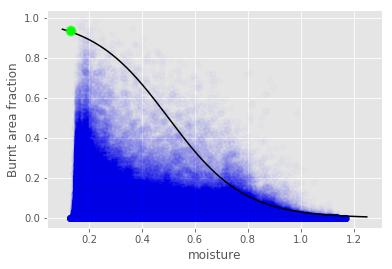
\includegraphics[width=5.78cm]{images/limitCurves/Desert/alphaVsFire}	
	\end{textblock*}
	\begin{textblock*}{14cm}(0.32cm,5cm)
		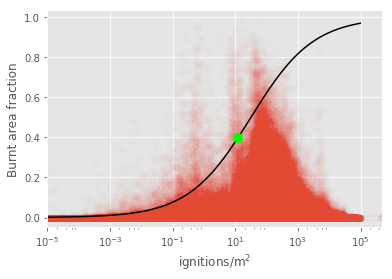
\includegraphics[width=5.78cm]{images/limitCurves/Desert/ignitionsVsFire.png}		
	\end{textblock*}
	\begin{textblock*}{14cm}(6.5cm,5.3cm)
		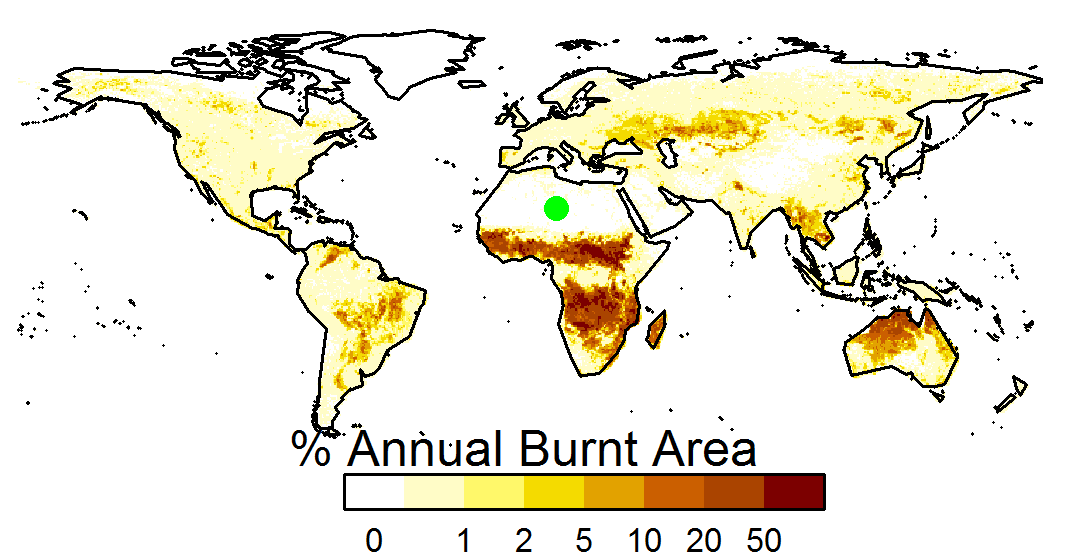
\includegraphics[width=5.78cm]{images/limitCurves/Desert/fireMap.png}		
	\end{textblock*}
\end{frame}
\addtocounter{framenumber}{-1}

\begin{frame}
	\frametitle{Controls on fire}
	%\framesubtitle{Geographic controls}
	\begin{textblock*}{14cm}(0.3cm,1.2cm)
		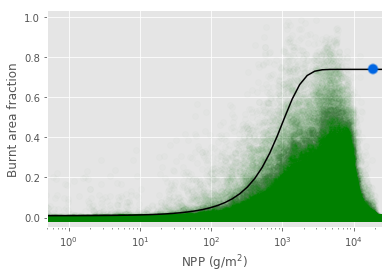
\includegraphics[width=5.78cm]{images/limitCurves/RainF/NPPVsFire}	
	\end{textblock*}
	\begin{textblock*}{14cm}(6.5cm,1.2cm)
		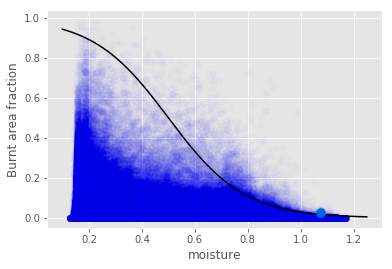
\includegraphics[width=5.78cm]{images/limitCurves/RainF/alphaVsFire}	
	\end{textblock*}
	\begin{textblock*}{14cm}(0.32cm,5cm)
		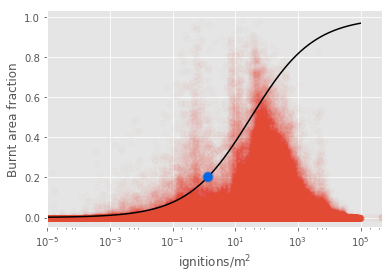
\includegraphics[width=5.78cm]{images/limitCurves/RainF/ignitionsVsFire.png}		
	\end{textblock*}
	\begin{textblock*}{14cm}(6.5cm,5.3cm)
		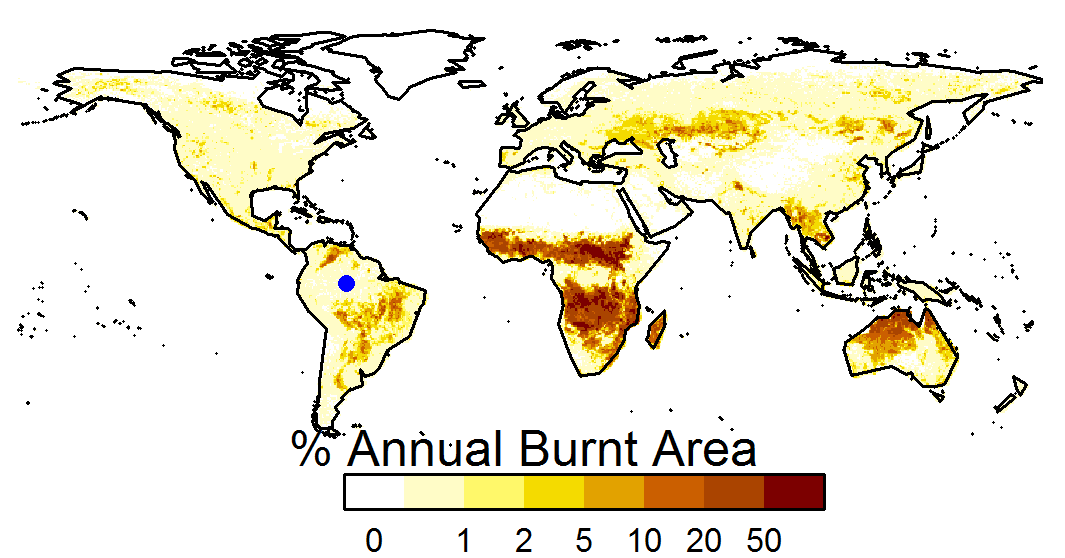
\includegraphics[width=5.78cm]{images/limitCurves/RainF/fireMap.png}		
	\end{textblock*}
\end{frame}
\addtocounter{framenumber}{-1}

\begin{frame}
	\frametitle{Controls on fire}
	%\framesubtitle{Geographic controls}
	\begin{textblock*}{14cm}(0.3cm,1.2cm)
		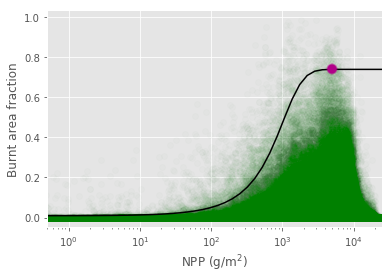
\includegraphics[width=5.78cm]{images/limitCurves/Savanna/NPPVsFire}	
	\end{textblock*}
	\begin{textblock*}{14cm}(6.5cm,1.2cm)
		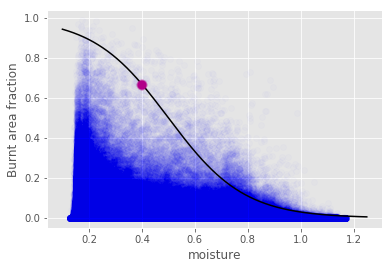
\includegraphics[width=5.78cm]{images/limitCurves/Savanna/alphaVsFire}	
	\end{textblock*}
	\begin{textblock*}{14cm}(0.32cm,5cm)
		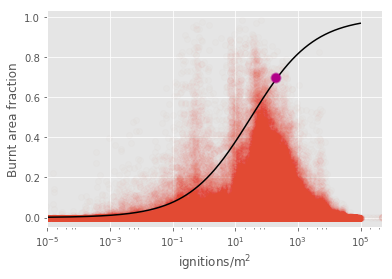
\includegraphics[width=5.78cm]{images/limitCurves/Savanna/ignitionsVsFire.png}		
	\end{textblock*}
	\begin{textblock*}{14cm}(6.5cm,5.3cm)
		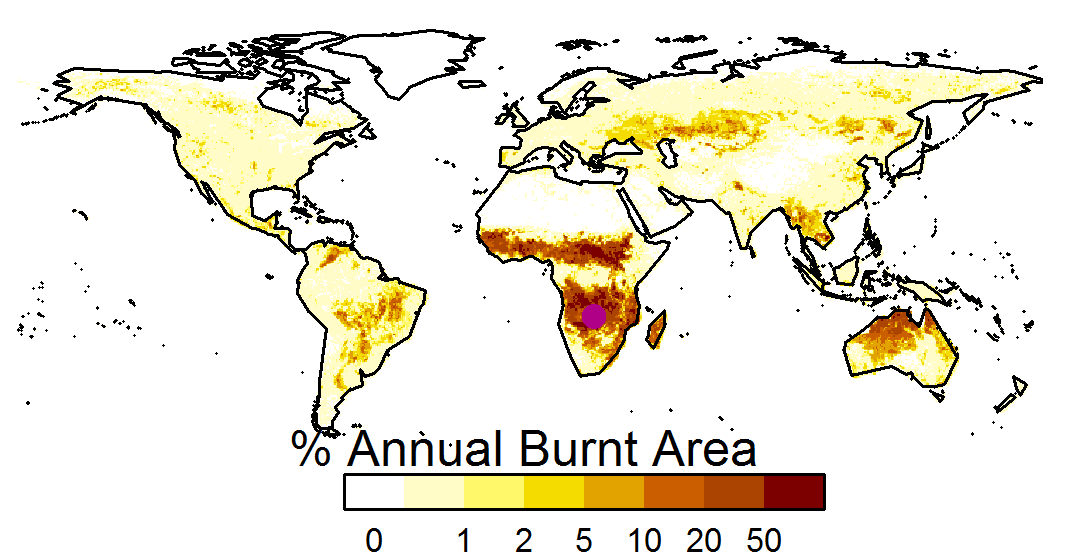
\includegraphics[width=5.78cm]{images/limitCurves/Savanna/fireMap.png}		
	\end{textblock*}
\end{frame}


\begin{frame}<1-3>[label=controlMapsNoLand]
    \frametitle{Controls on fire}
    %\framesubtitle{Geographic controls}
    
	\controlsSide{limitation_map_no_supression}
    
    \begin{textblock*}{14cm}(3.1cm,3.25cm)
    	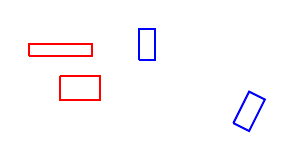
\begin{tikzpicture}
    \visible<3> {
    	% Sahel
    	\draw[red, line width = 0.25mm] (3.2,5.25) -- (4.0,5.25) -- (4.0,5.4) -- (3.2,5.4) -- (3.2,5.25);
    	
    	\draw[red, line width = 0.25mm] (3.6,5.0) -- (4.1,5.0) -- (4.1,4.7) -- (3.6,4.7) -- (3.6,5.0);
    }
	 \visible<4> {
	 	\draw[blue, line width = 0.25mm] (4.6,5.2) -- (4.8,5.2) -- (4.8,5.6) -- (4.6,5.6) -- (4.6,5.2);
	 	
	 	\draw[blue, line width = 0.25mm] (5.8,4.4) -- (6.0,4.3) -- (6.2,4.7) -- (6.0,4.8) -- (5.8,4.4);
	 }
	\end{tikzpicture}
	\end{textblock*}
	\begin{textblock*}{14cm}(6.7cm,1.45cm)
		\only<3->{
		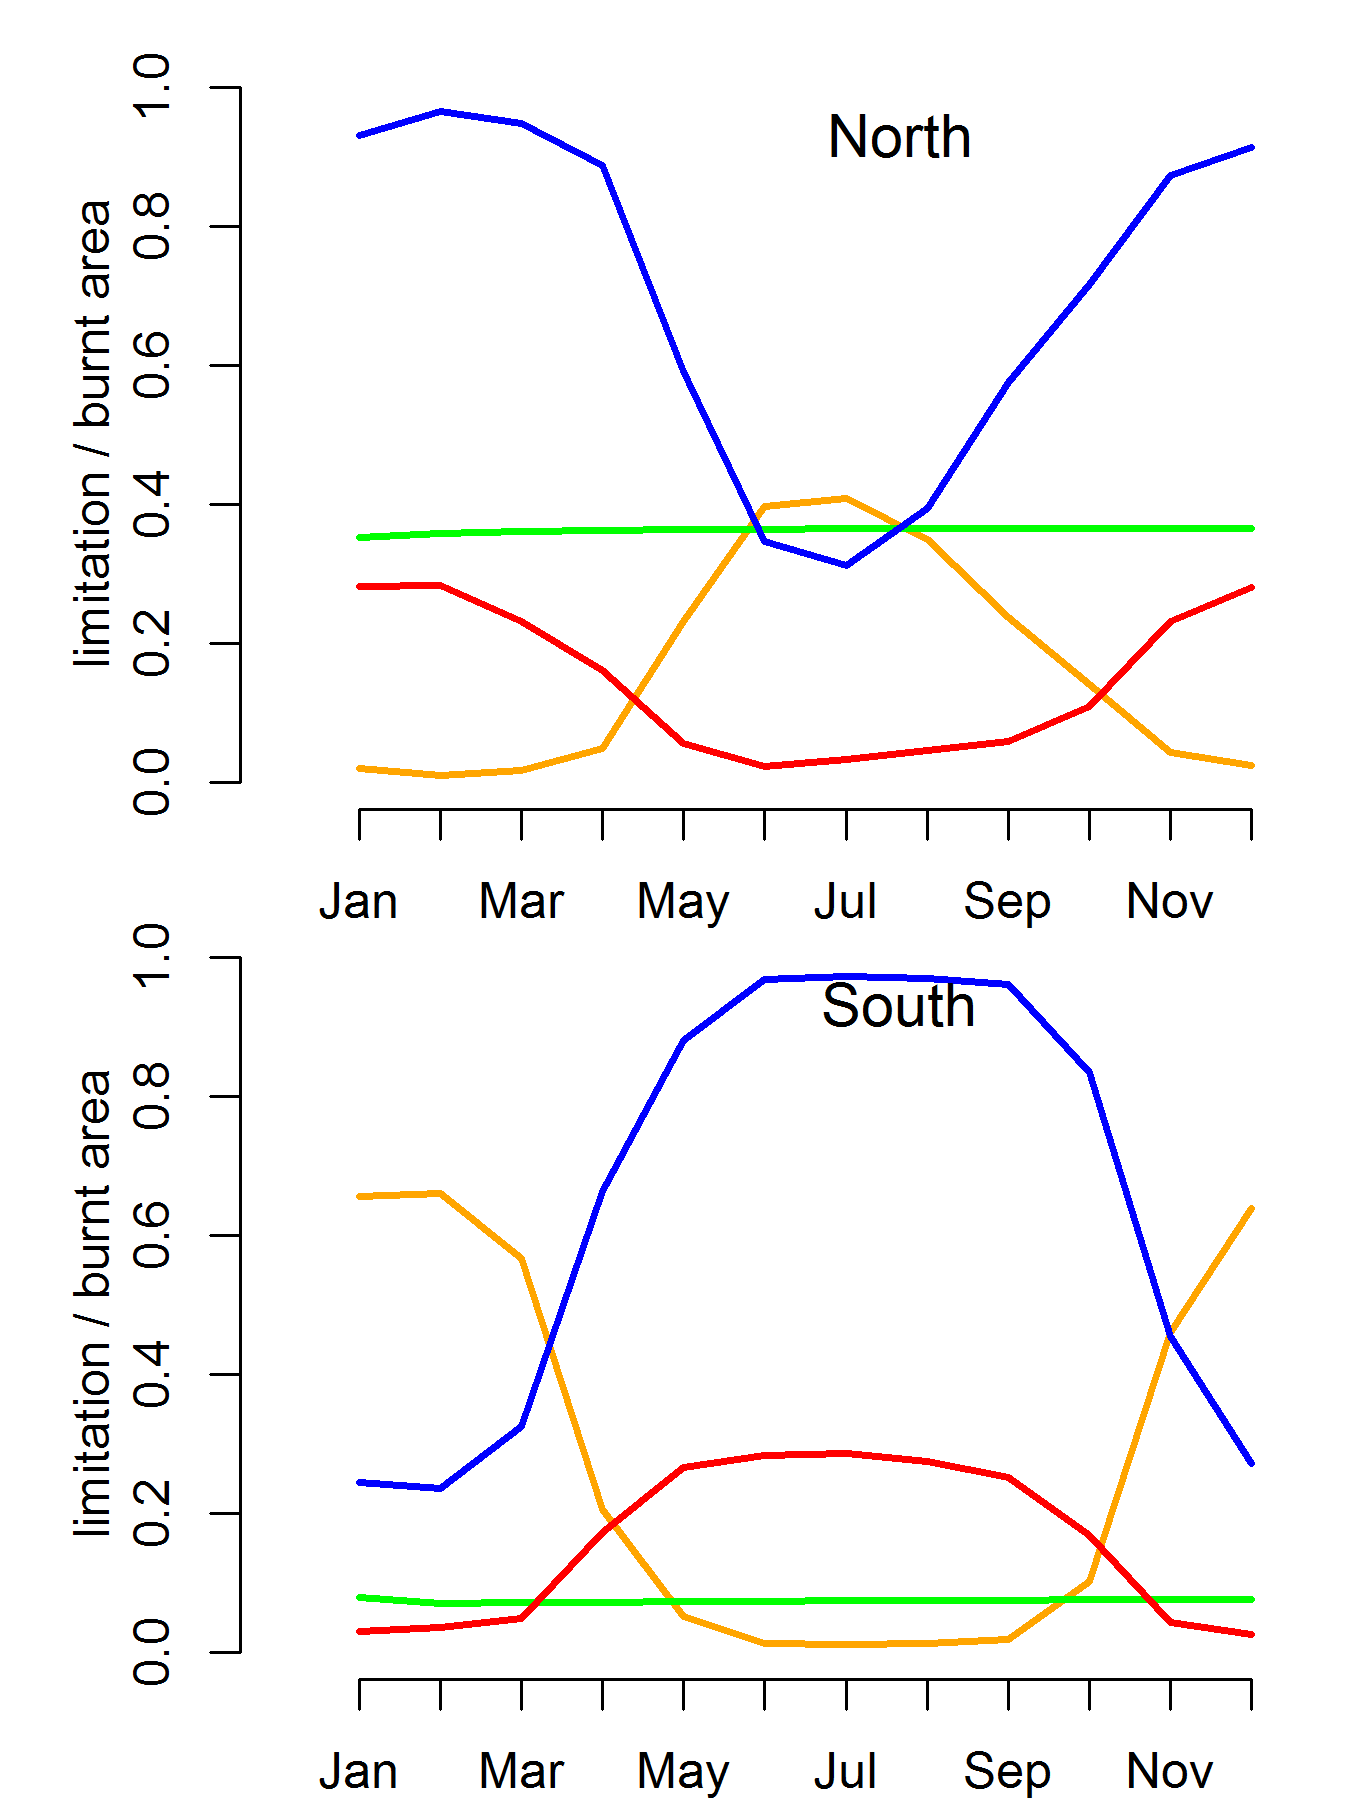
\includegraphics[width=5.7cm]{images/caseStudy/seasonal_casestudyAfrica}}
		\only<4->{
			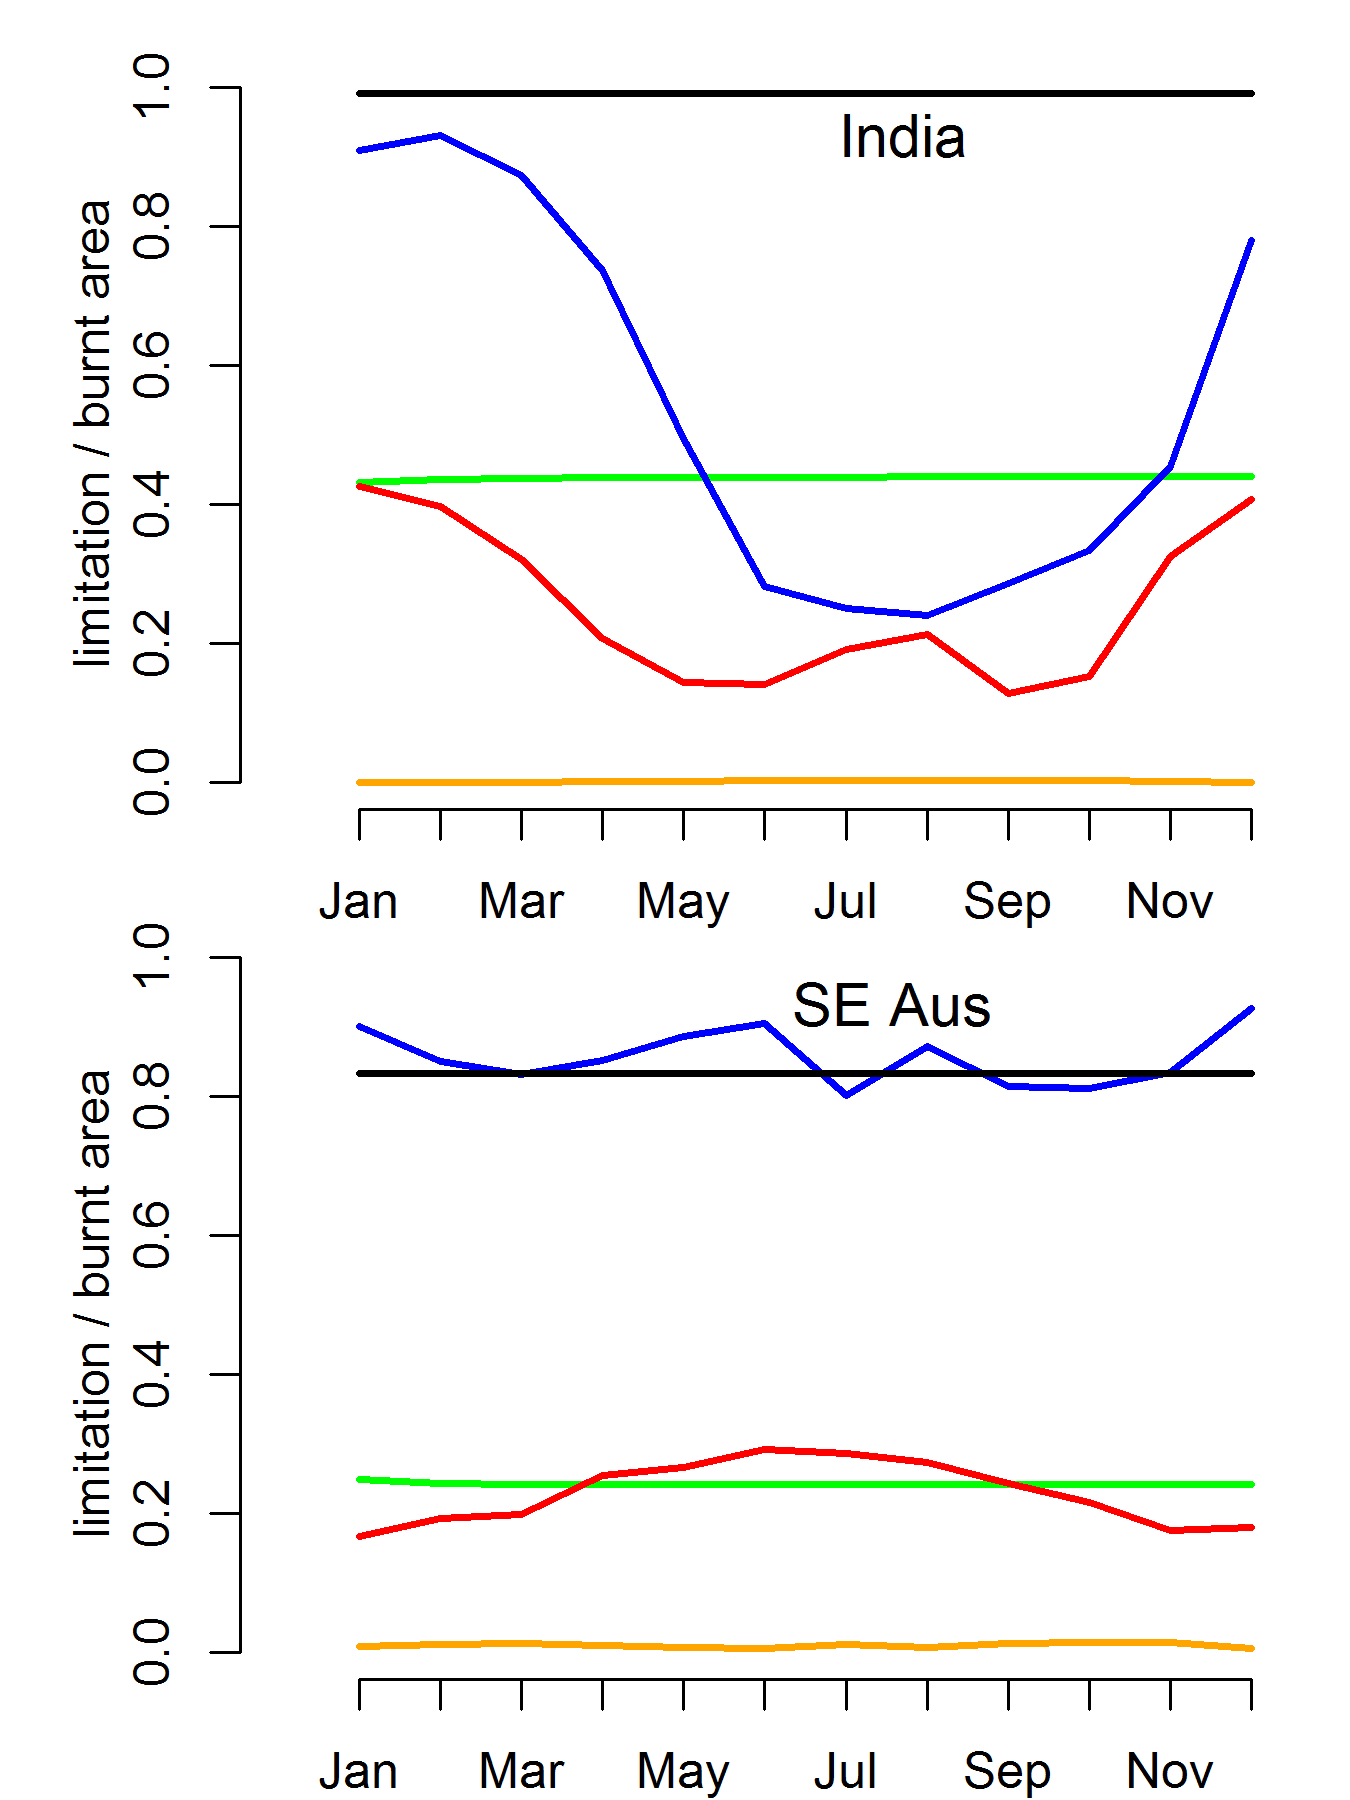
\includegraphics[width=5.7cm]{images/caseStudy/seasonal_casestudyAsia1}}
	\end{textblock*}
\end{frame}

\section{Ignitions}

\begin{frame}
    \frametitle{Igntions}
    \framesubtitle{Just Humans, Just natural, both combined}


\end{frame}

\begin{frame}
    \frametitle{Igntions}
    \framesubtitle{Igntion saturattion and manipulation}


\end{frame}

\section{Fragmentation}

\pgfdeclareimage[width=1.0\paperwidth]{header-image}{header_images/helicopter}
\againframe<6->{framework}


\begin{frame}<2>[label=controlMaps]
    \frametitle{So Humans have no impact on fire?}
    \framesubtitle{Suppression \& Fragmentation}
    \controlsSide{limitation_map_no_supression_light}
\end{frame}

\addtocounter{framenumber}{-1}
\begin{frame}<2>[label=controlMaps]
	\frametitle{So Humans have no impact on fire?}
	\framesubtitle{Suppression \& Fragmentation}
	\controlsSide{limitation_map_light}
\end{frame}

\addtocounter{framenumber}{-1}
\begin{frame}<2>[label=controlMaps]
	\frametitle{So Humans have no impact on fire?}
	\framesubtitle{Suppression \& Fragmentation}
	\controlsSide{limitation_map_noColour}
\end{frame}

\addtocounter{framenumber}{-1}
\begin{frame}<2-4>[label=controlMaps]
	\frametitle{So Humans have no impact on fire?}
	\framesubtitle{Suppression \& Fragmentation}
	\controlsSide{limitation_map_light}
	
	\begin{textblock*}{14cm}(3.1cm,3.25cm)
		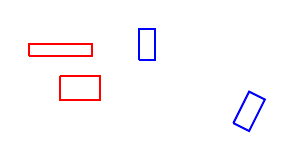
\begin{tikzpicture}
		\visible<5> {
			% Sahel
			\draw[red, line width = 0.25mm] (3.2,5.25) -- (4.0,5.25) -- (4.0,5.4) -- (3.2,5.4) -- (3.2,5.25);
			
			\draw[red, line width = 0.25mm] (3.6,5.0) -- (4.1,5.0) -- (4.1,4.7) -- (3.6,4.7) -- (3.6,5.0);
		}
		\visible<3-> {
			\draw[blue, line width = 0.25mm] (4.6,5.2) -- (4.8,5.2) -- (4.8,5.6) -- (4.6,5.6) -- (4.6,5.2);
			
			\draw[blue, line width = 0.25mm] (5.8,4.4) -- (6.0,4.3) -- (6.2,4.7) -- (6.0,4.8) -- (5.8,4.4);
		}
		\end{tikzpicture}
	\end{textblock*}
	\begin{textblock*}{14cm}(6.7cm,1.45cm)
		
		\only<3>{
			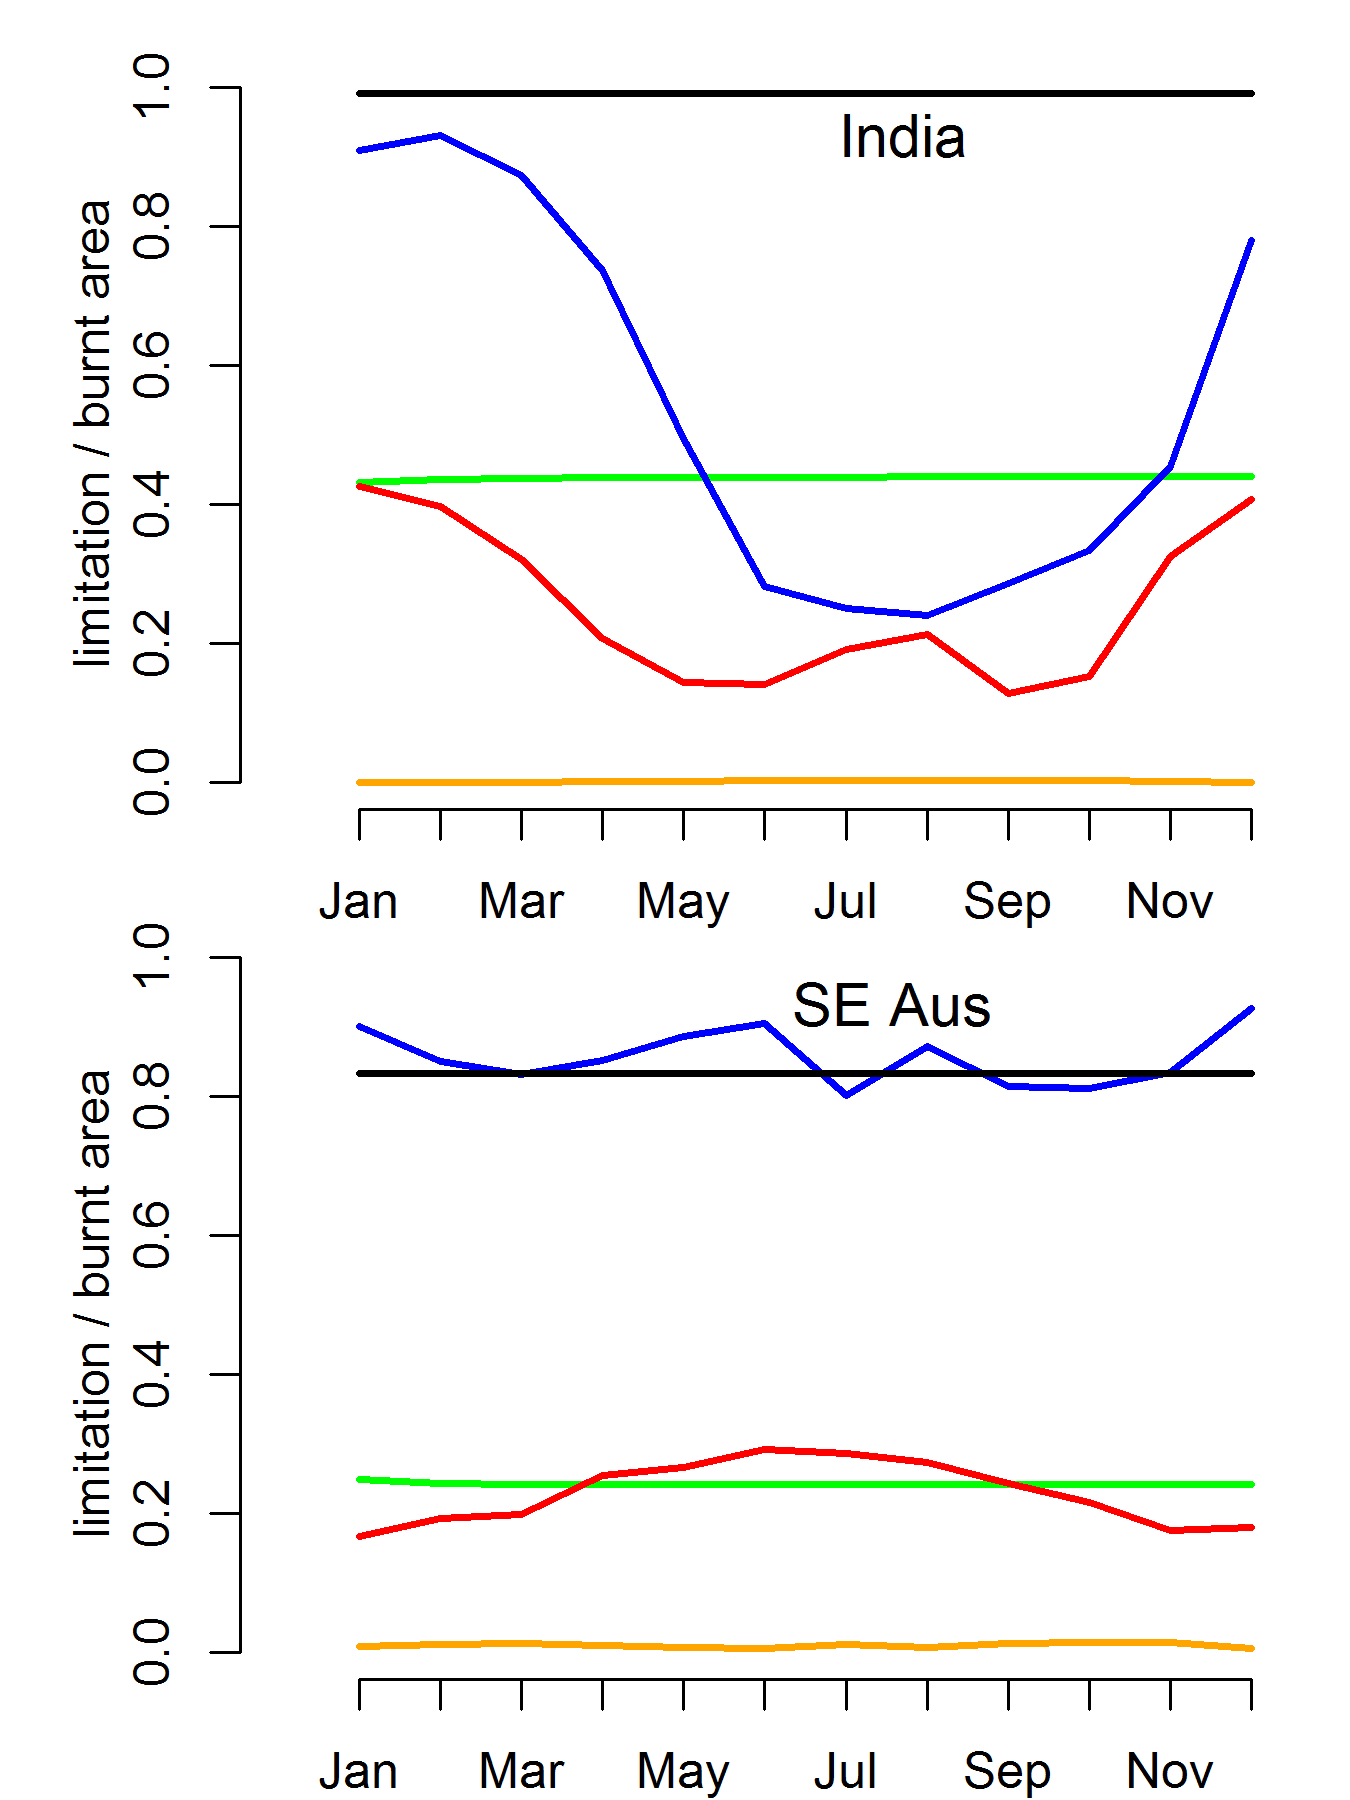
\includegraphics[width=5.7cm]{images/caseStudy/seasonal_casestudyAsia1}}
		\only<4>{
			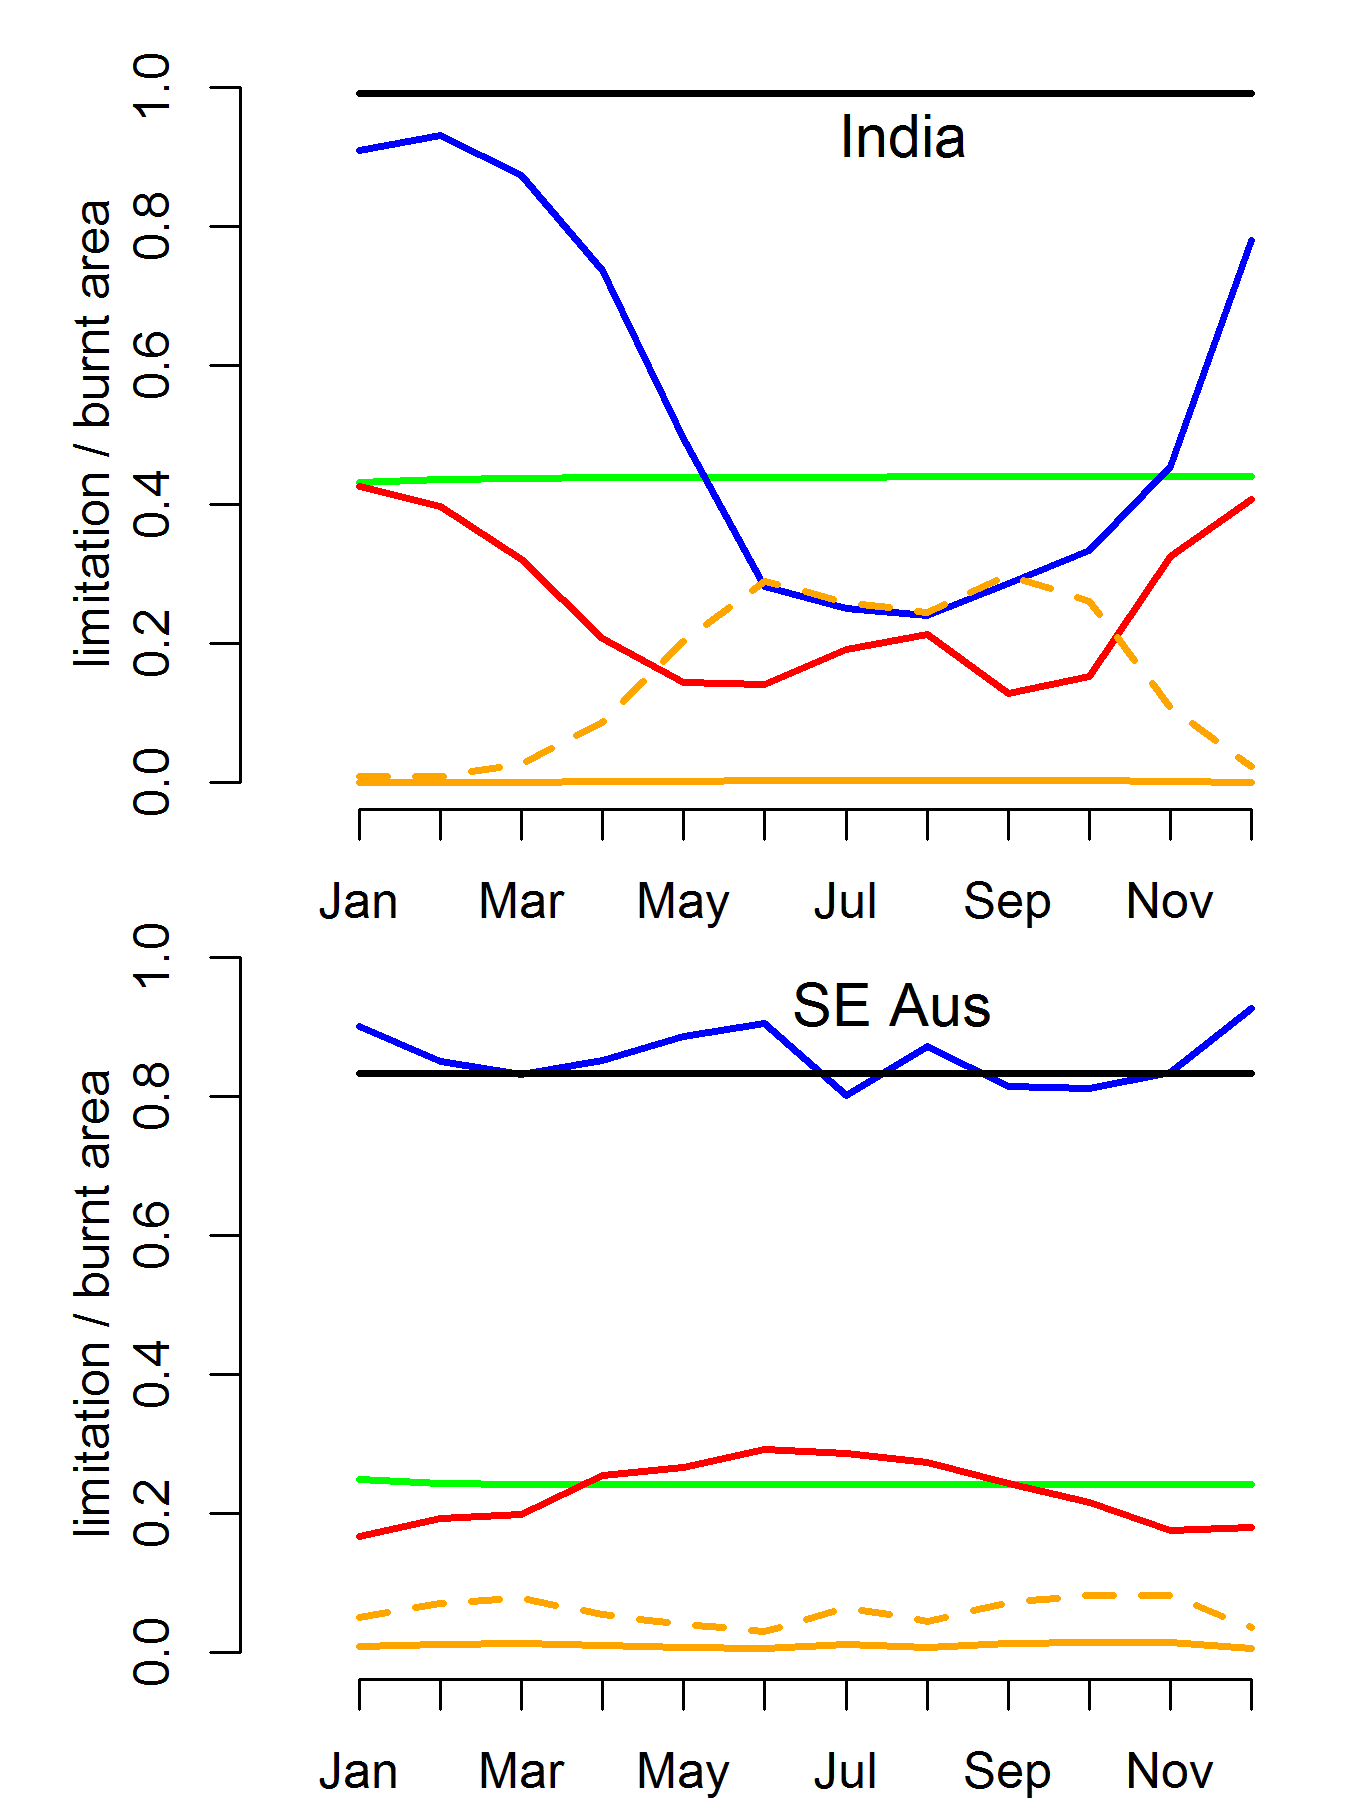
\includegraphics[width=5.7cm]{images/caseStudy/seasonal_casestudyAsia2}}
	\end{textblock*}
	
\end{frame}

\pgfdeclareimage[width=1.0\paperwidth]{header-image}{header_images/Mirador_de_Garbi}
\begin{frame}
    \frametitle{So Humans have no impact on fire?}
    \framesubtitle{Suppression \& Fragmentation}
    \begin{textblock*}{11cm}(0cm,1.5cm)
    \visible<1->{
    	\begin{tikzpicture}
    	\node[anchor=north,inner sep=0] (image) at (0,0) {
    		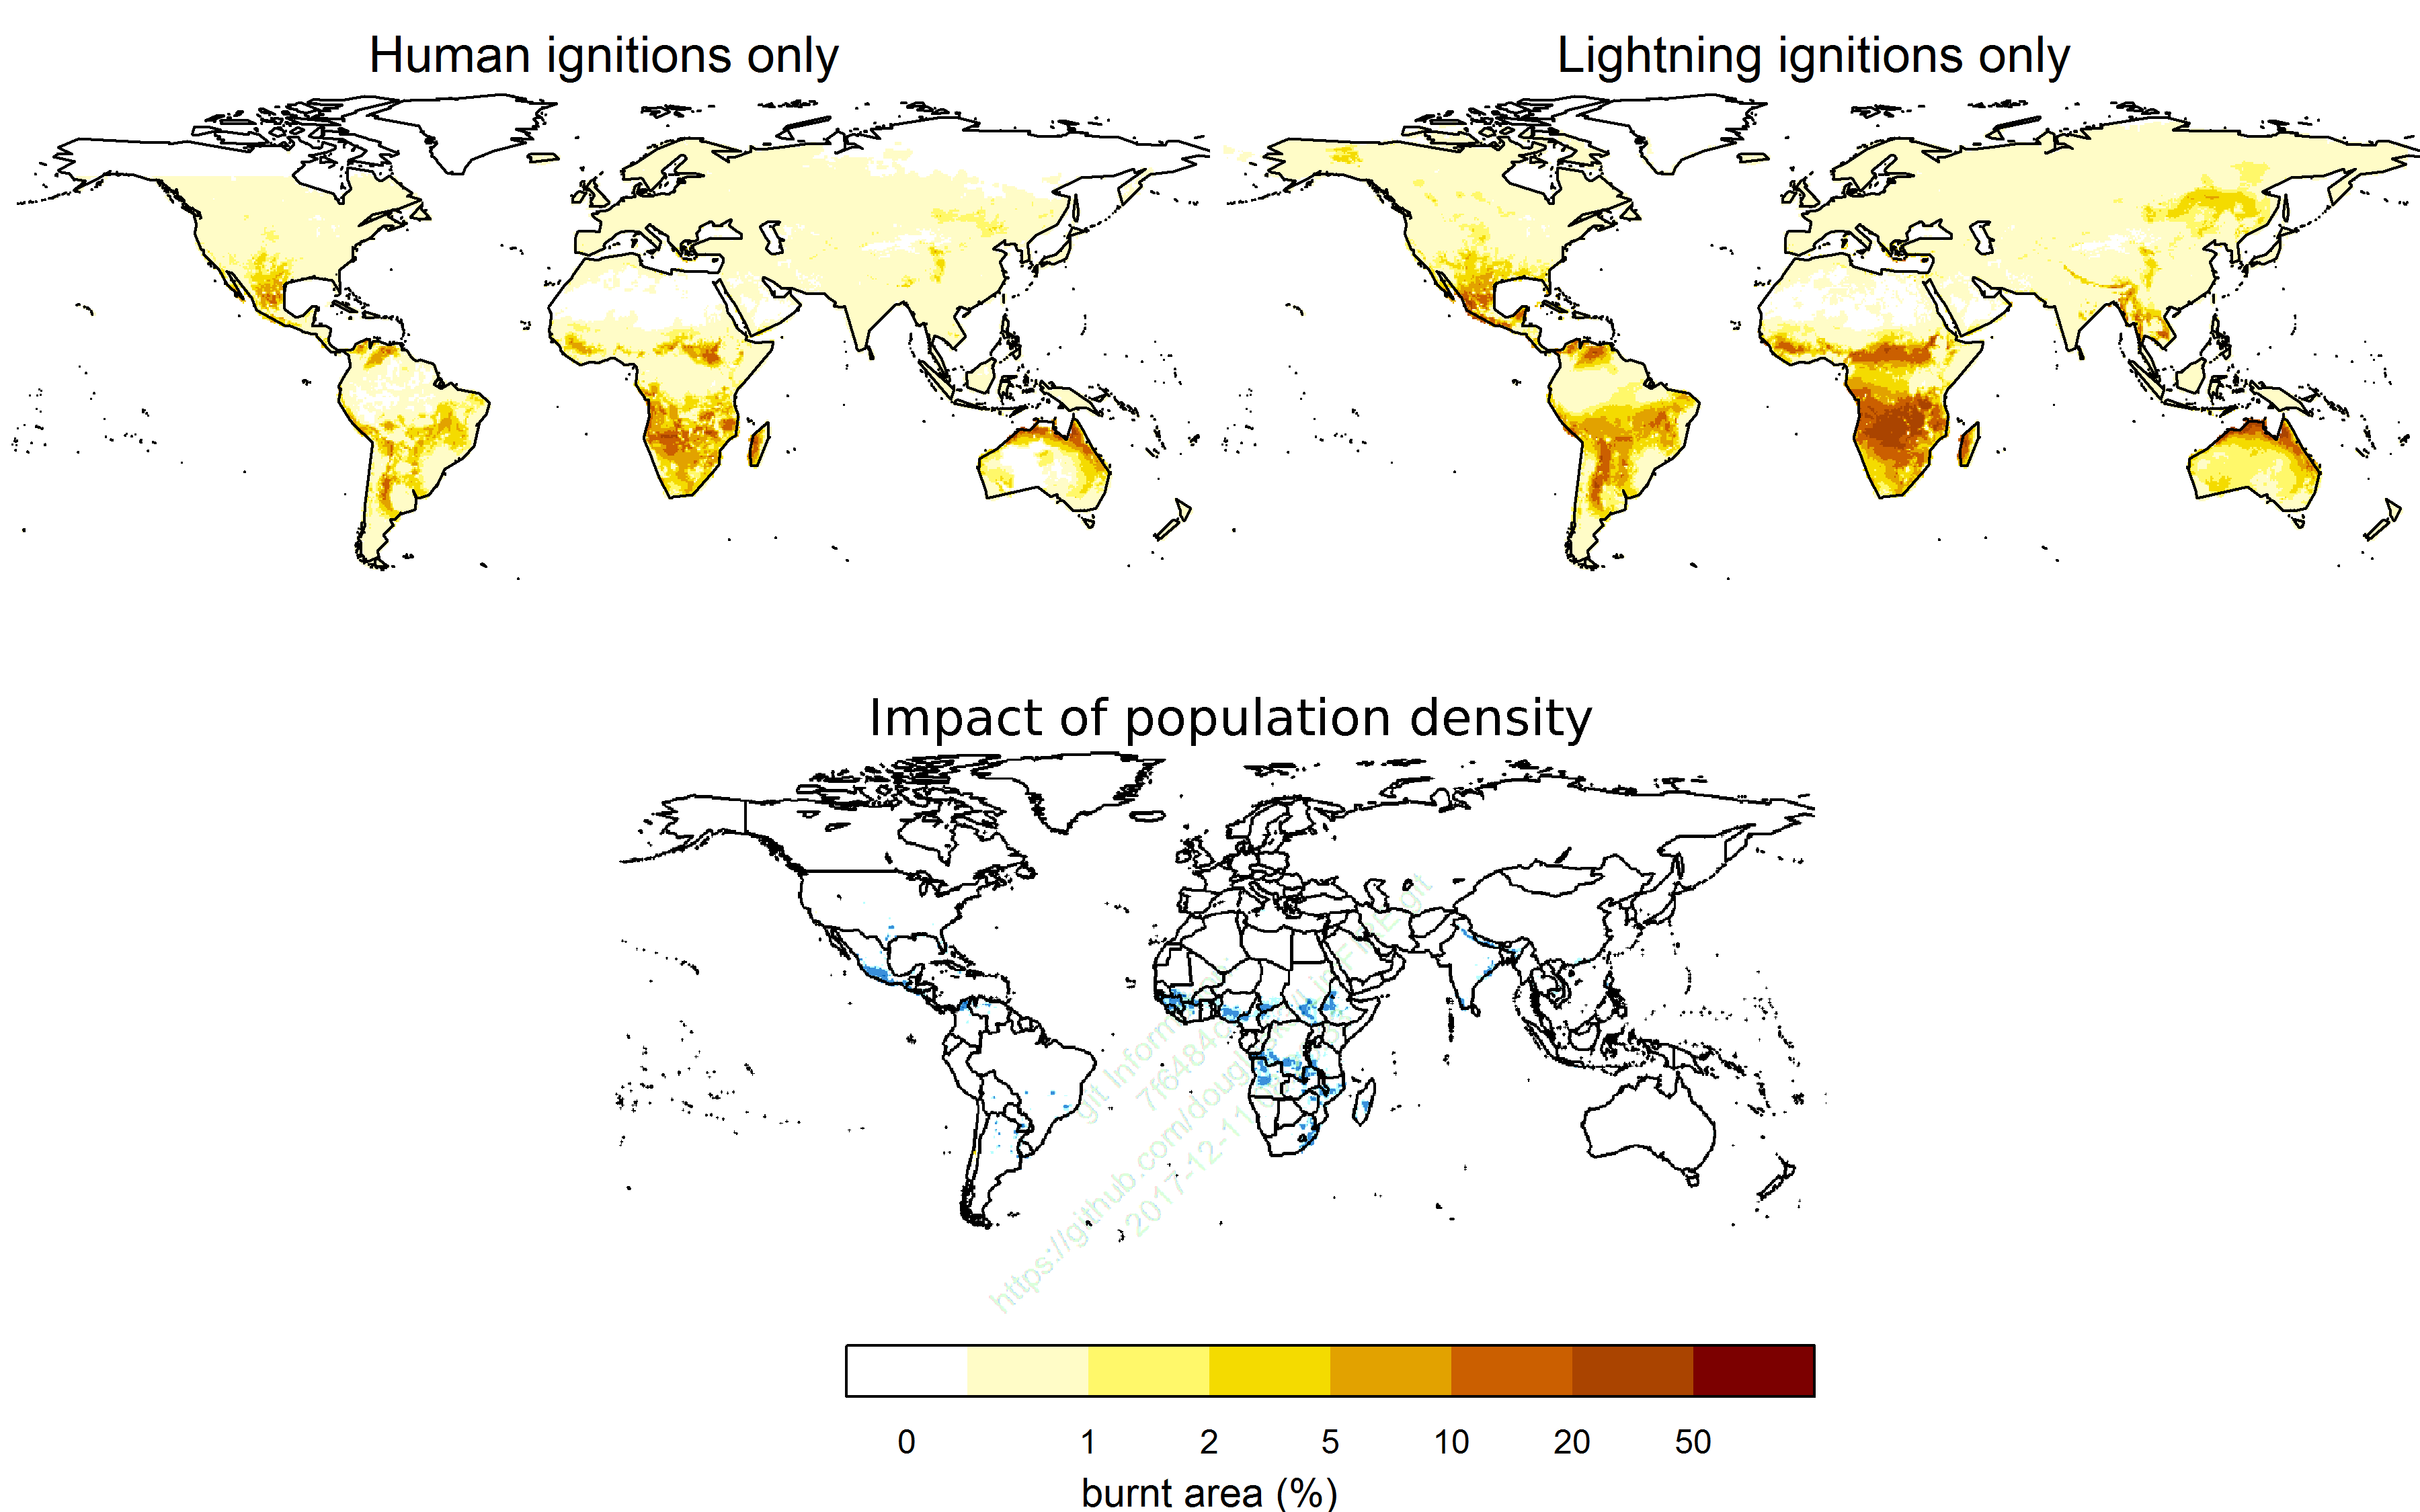
\includegraphics[trim={5.1cm 2cm 5.1cm 6.2cm},clip,width=6.2cm]{images/igntitions/IgntionInfoSourceAdding}
	    };
        \node[anchor=south,align=center] at (0, -0.2) {Human Ignitions};
        \end{tikzpicture}
    }
	%trim = {l b r t}
    \visible<1->{
    	\begin{tikzpicture}
    	\node[anchor=north,inner sep=0] (image) at (0,0) {
    		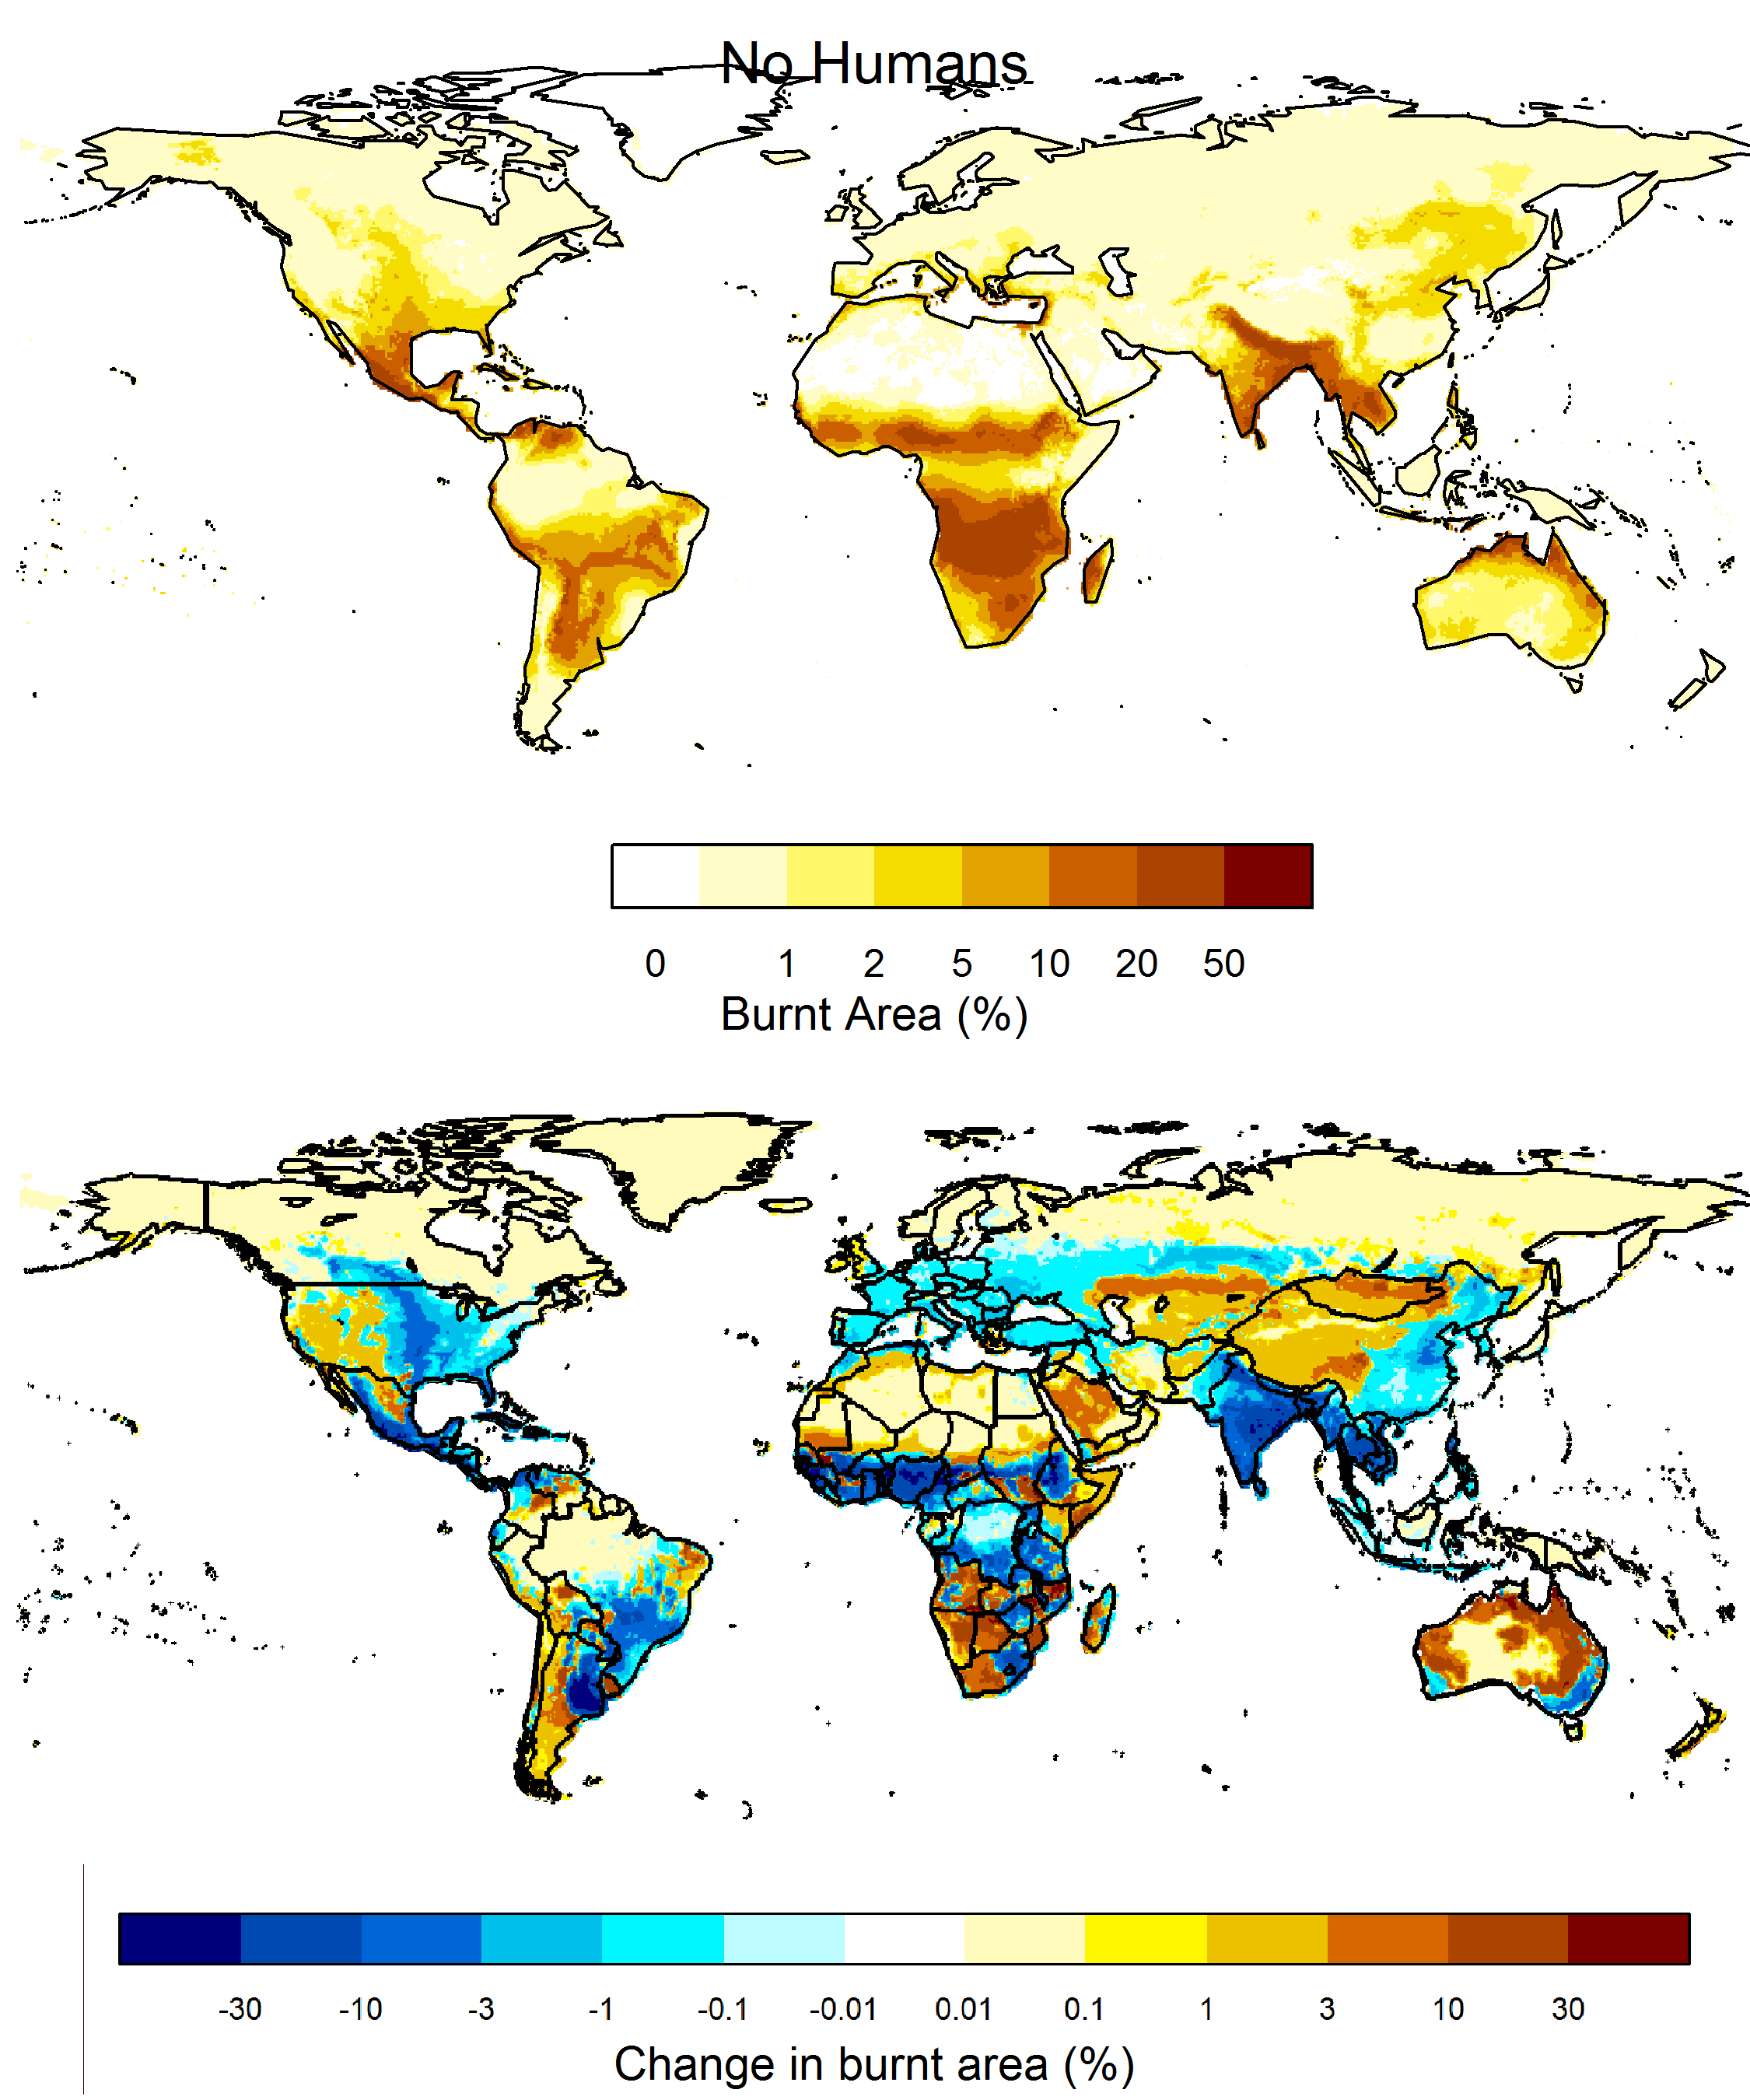
\includegraphics[trim={0 0 0 8cm},clip,width=6.2cm]{images/igntitions/IgntionInfoNoHumans}
    	};
    	\node[anchor=south,align=center] at (0, -0.2) {Overall Human Impact};
    	\end{tikzpicture}
        
    }
    \end{textblock*}
    \begin{textblock*}{11cm}(6.4cm,1.3cm)
    \visible<2->{
        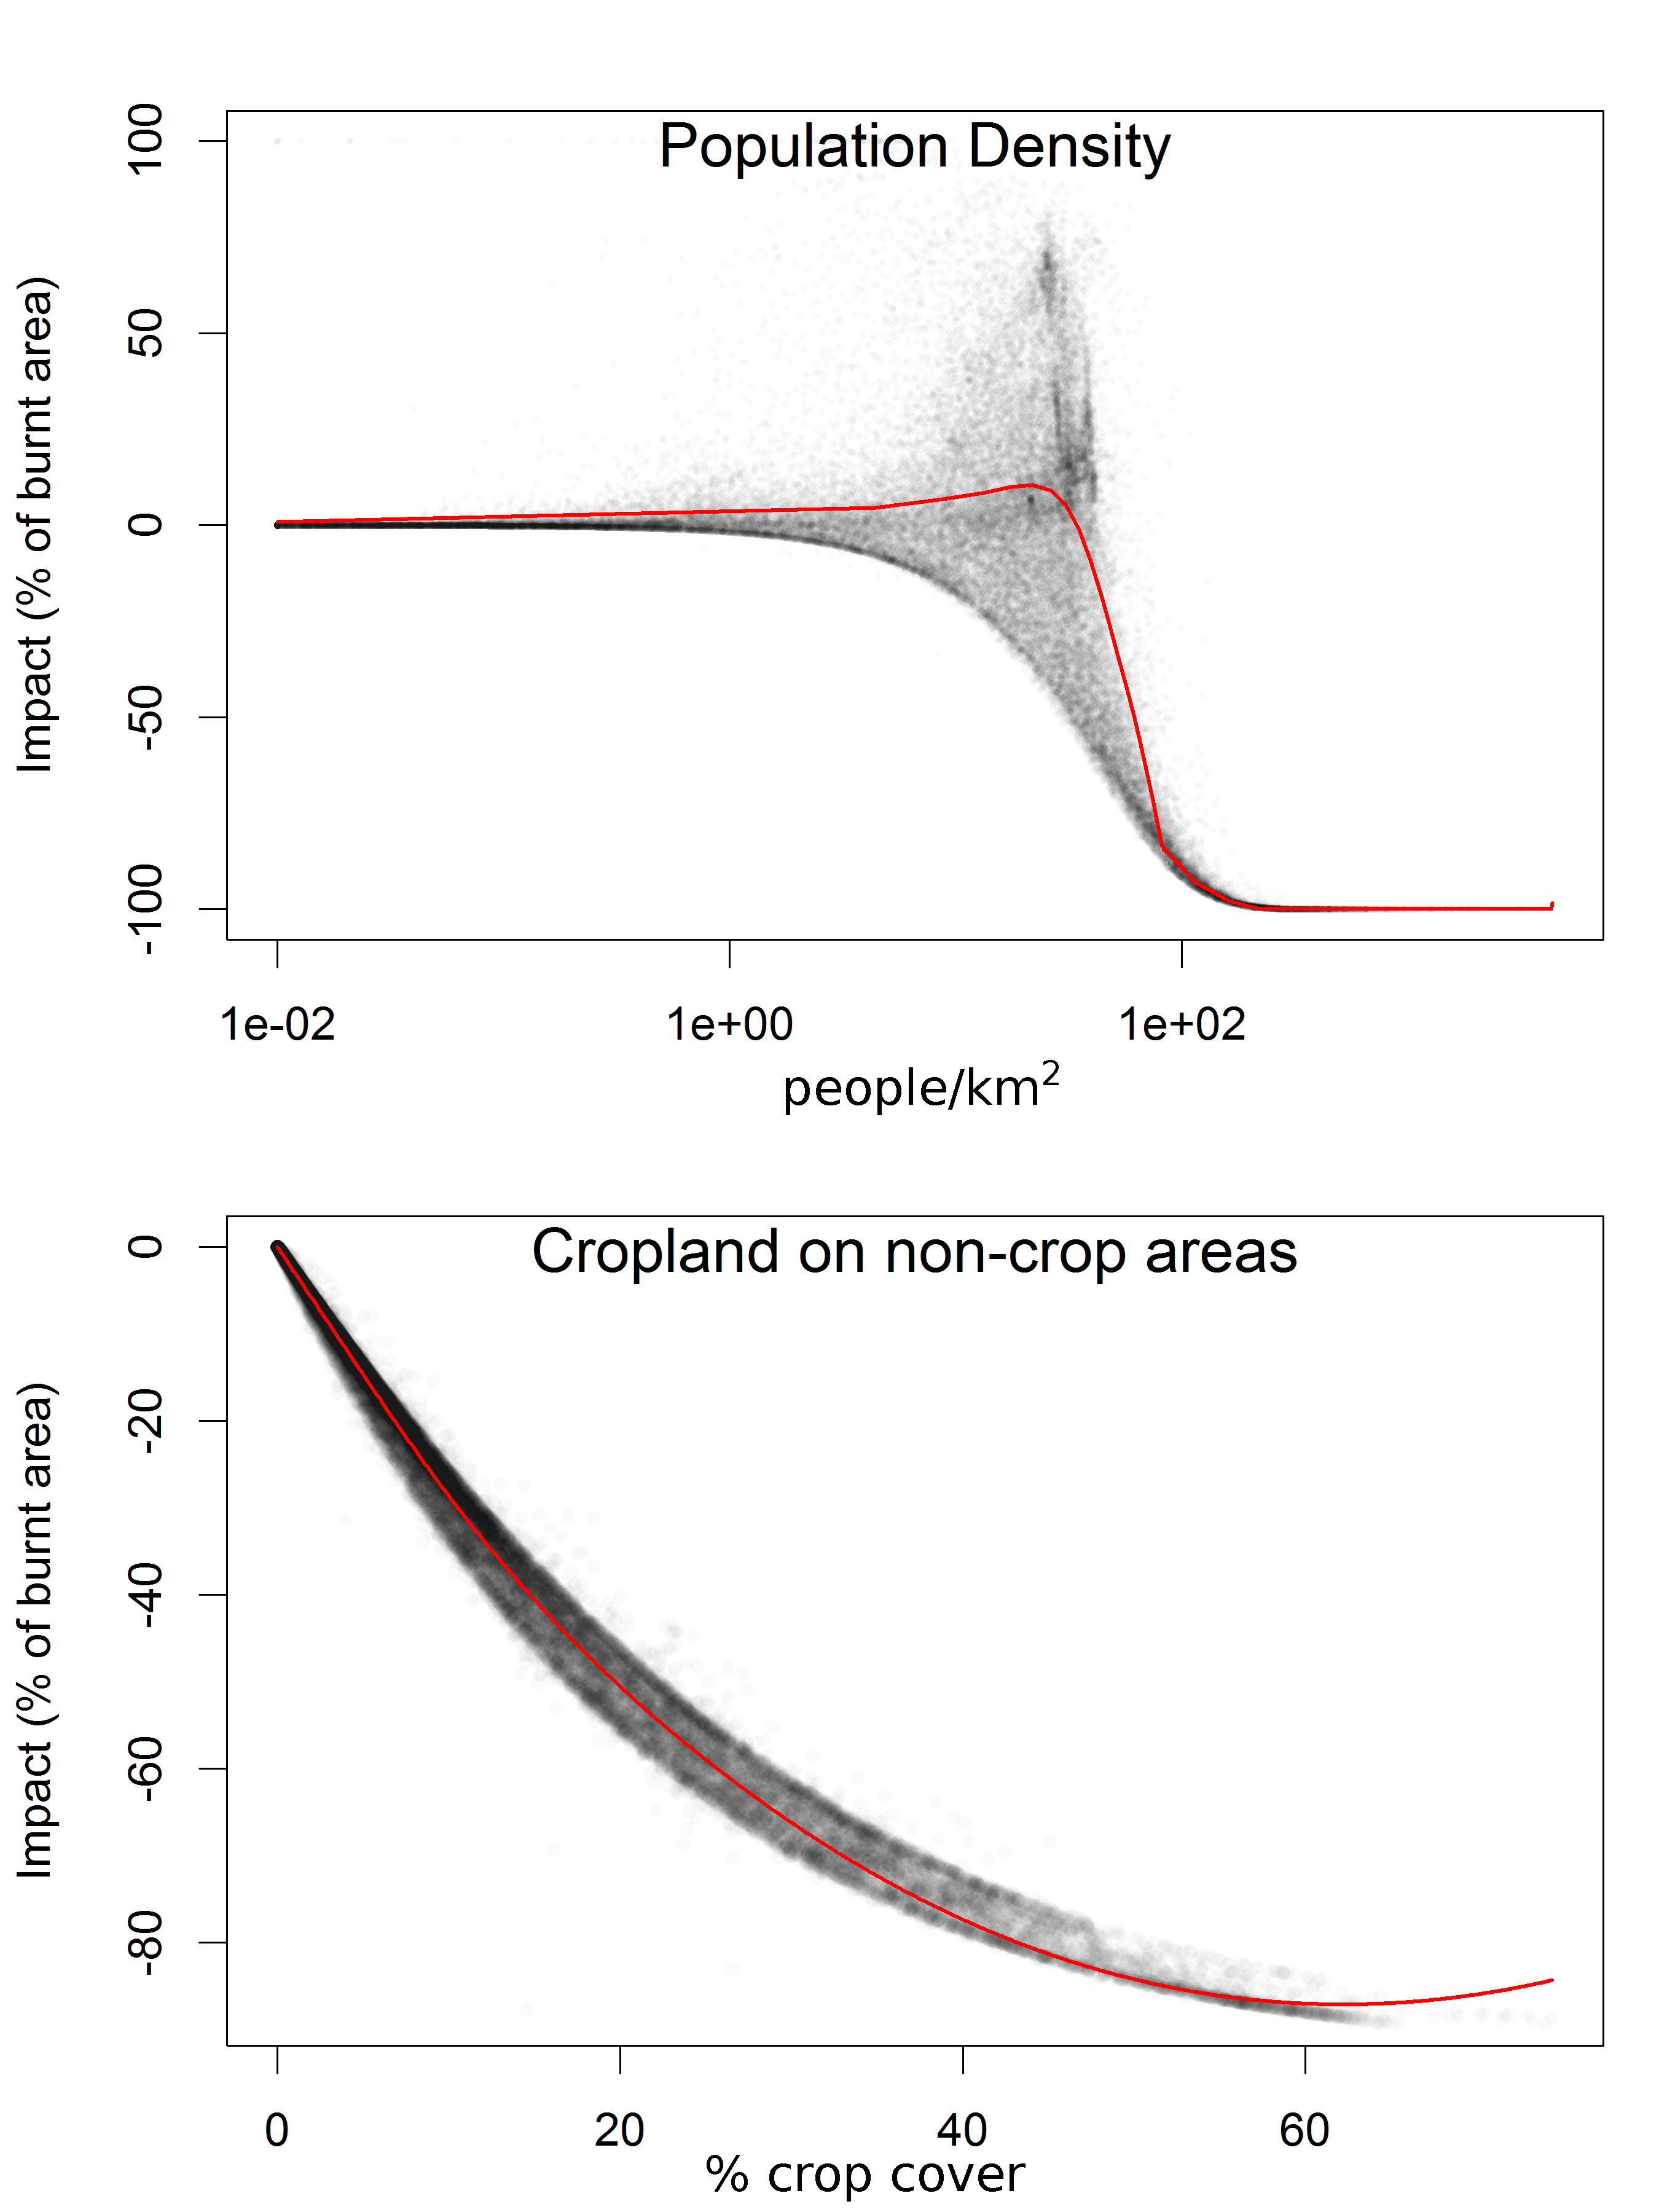
\includegraphics[width=5.5cm]{images/human_noHuman_impact}
    }
    \end{textblock*}

    %\visible<3->{
    %    \begin{tikzpicture}
    %        \node[anchor=south west,inner sep=0] (image) at (0,0) {
    %            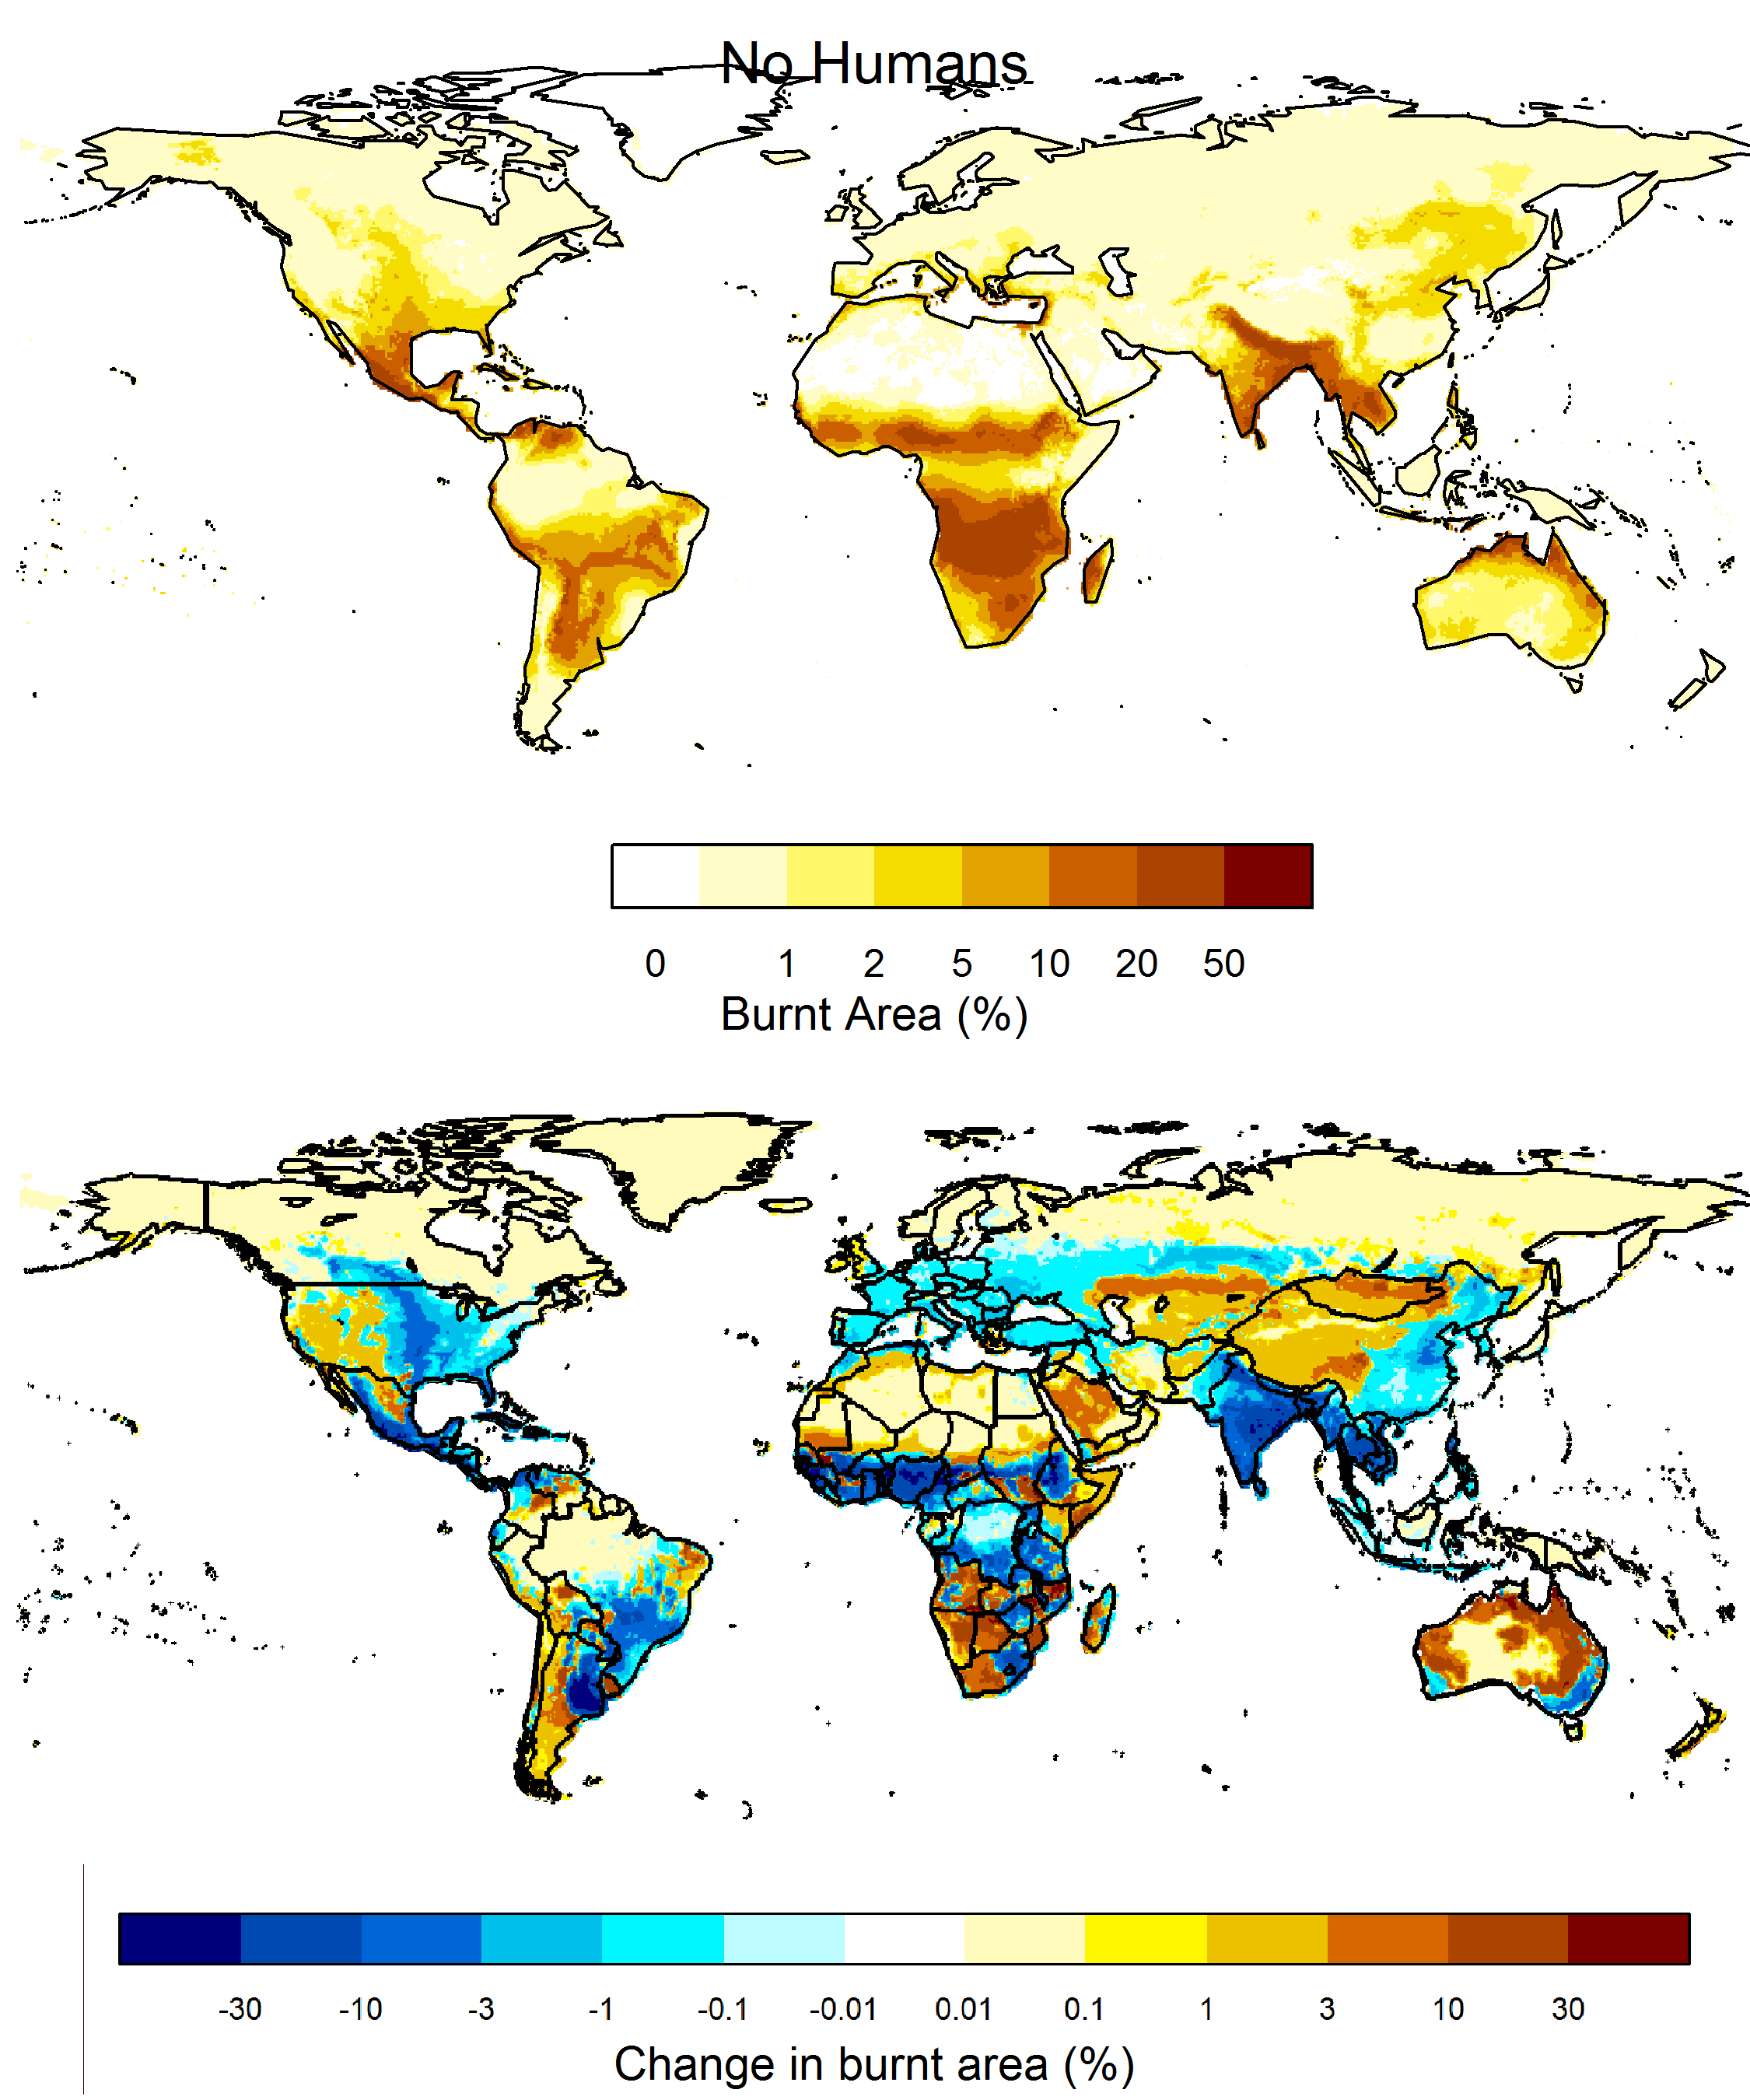
\includegraphics[trim={0 0 0 8cm},clip,width=11.0cm]{images/igntitions/IgntionInfoNoHumans}
    %        };
    %
            %\visible<-1> {\draw[white, fill = white] (5.5,4) -- (12.0,4) -- (12.0,0.0) -- (5.5,0.0) -- (5.5,4);}
    %    \end{tikzpicture}
    %}
\end{frame}

\pgfdeclareimage[width=1.0\paperwidth]{header-image}{header_images/firefighter}

%\begin{frame}<2-3>
%    \frametitle{Sensitivity to Controls}
%    \controlsSide{limitation_map}
%\end{frame}

\section{Conclusion}

\pgfdeclareimage[width=1.0\paperwidth]{header-image}{header_images/post_fire}

\begin{frame}
    \frametitle{Humans reduce burnt area}
    %Conclusions
    %Caviats
\end{frame}

%\section{Example slides}

\begin{frame}
  \frametitle{Prerequisites \& Goals}
  \framesubtitle{Knowledge is a brick wall that you raise line by line forever}
  \begin{block}{LaTeX}
  \begin{itemize}
    \item Obviously some basic LaTeX knowledge is necessary
    \item Some more features will be provided here
  \end{itemize}
  \end{block}

  \begin{block}{Beamer}
  \begin{itemize}
    \item You'll learn them by looking at this presentation source
  \end{itemize}
  \end{block}

  \begin{block}{Goal}
  \begin{itemize}
    \item Learn how to make well structured slides
    \item Using a beautiful theme (congrats to the Oxygen team!)
    \item Take over the world
    \item Relax...
  \end{itemize}
  \end{block}
\end{frame}

\section{Basic structuring}
\begin{frame}
  \frametitle{Sections, Frames and Blocks}
  \framesubtitle{Put everything into boxes}

  The current section is "Basic structuring". And the current frame
  is what you have on the screen right now.

  \begin{block}{A beautiful block}
  A block has a title, and some content. You can put in a block
  almost everything you want that is provided by LaTeX. For example
  math works as usual:
    \begin{equation}
    \sum_{i=1}^n i = \frac{n \times (n+1)}{2}
    \end{equation}
  \end{block}

  Also works outside a block:
  \begin{equation}
  \sum_{i=1}^n i^2 = \frac{n \times (n+1) \times (2n+1)}{6}
  \end{equation}
\end{frame}

\begin{frame}
  \frametitle{Different type of blocks}
  \framesubtitle{Weeeee! Colors!!}
  \begin{block}{Standard block}
  \begin{itemize}
    \item A standard block, used for grouping
    \item Obviously can contain itemizes too...
    \begin{itemize}
      \item And nested itemizes...
      \item of course!
    \end{itemize}
  \end{itemize}
  \end{block}
  \begin{alertblock}{Alert block}
  WARNING: Something very important inside this block!
  \end{alertblock}
  \begin{example}
  Note that examples are displayed as a special block...
  \end{example}
\end{frame}

\section{Fancy features}
\begin{frame}
  \frametitle{Highlighting}
  \framesubtitle{Hey! Look here! here!}

  \begin{block}{A regular block}
  \begin{itemize}
    \item Normal text
    \item \highlighton{Highlighted text} to draw attention
    \item \alert{"Alert'ed" text} to spot very important information
    \item Alternatively you can
    \begin{itemize}
      \alert{\item "Alert" the item itself}
      \highlighton{\item Or "Highlight" it}
    \end{itemize}
  \end{itemize}
  \end{block}
  \begin{alertblock}{If it's very very important...}
  \alert{... you can "alert" in an "alertblock"}\\
  Ewww, nasty, heh?
  \end{alertblock}
\end{frame}

\newcommand{\putlink}[1]{%
   \pgfsetlinewidth{1.4pt}%
   \pgfsetendarrow{\pgfarrowtriangle{4pt}}%
   \pgfline{\pgfxy(1,1)}{\pgfxy(#1,1)}
}

\begin{frame}
  \frametitle{Overlay effects}
  \framesubtitle{Keep the suspense!}
  \begin{block}{Time bomb}
  \begin{enumerate}
    \item<2-> Two more to go
    \item<3-> One more to go
    \item<4-> Last chance...
    \item<5-> BOOM!
  \end{enumerate}
  \end{block}
  \begin{block}{"Animation"}<6->
    \begin{pgfpicture}{0cm}{0cm}{7cm}{2cm}
    \only<1-6>{
      \putlink{2}
    }
    \only<7>{
      \putlink{4}
    }
    \only<8>{
      \putlink{6}
    }
    \only<9>{
      \putlink{8}
    }
    \only<10>{
      \putlink{10}
    }
    \end{pgfpicture}
  \end{block}
\end{frame}

\section*{}
\frame{
  \vfill
  \centering
  \highlighton{
  \usebeamerfont*{frametitle}And now?

  \usebeamerfont*{framesubtitle}Enter the secret section
  }
  \vfill
}
\begin{frame}
  \frametitle{Contributing to this beamer style}
  \framesubtitle{We want you !}

  \begin{block}{Why?}
  \begin{itemize}
    \item Beamer is hot!
    \item This style deserves to be improved
  \end{itemize}
  \end{block}

  \begin{block}{How?}
  \begin{itemize}
    \item Grab it
    \item Improve its LaTeX code
    \item Use you artistics skills
    \item Document it
    \item Help other people to use it
    \item Use it...
  \end{itemize}
  \end{block}
\end{frame}

\begin{frame}
  \frametitle{Resources}
  \framesubtitle{If you want to improve this style}
  \begin{thebibliography}{10}

  \beamertemplatearticlebibitems

  \bibitem{beamer-homepage}
    LaTeX Beamer
    \newblock {\tt http://latex-beamer.sourceforge.net/}

  \bibitem{kdeslides}
    KDE Presentations
    \newblock {\tt http://www.kde.org/kdeslides/}

  \end{thebibliography}
\end{frame}

\frame{
  \vspace{2cm}
  {\huge Questions ?}

  \vspace{3cm}
  \begin{flushright}
    Konqi Konqueror

    \structure{\footnotesize{konqi@kde.org}}
  \end{flushright}
}


\end{document}
